\documentclass[10pt, portrait]{article}
\usepackage[scaled=0.92]{helvet}
\usepackage{calc}
\usepackage{multicol}
\usepackage{ifthen}
\usepackage[a4paper,margin=5mm,portrait]{geometry}
\usepackage{amsmath,amsthm,amsfonts,amssymb}
\usepackage{physics}
\usepackage{color,graphicx,overpic}
\usepackage{hyperref}
\usepackage{newtxtext} 
\usepackage{enumitem}
\usepackage{amssymb}
\usepackage[table]{xcolor}
\usepackage{vwcol}
\usepackage{tikz}
\usetikzlibrary{arrows.meta,calc,angles,quotes}
\usepackage{mathtools}
\usepackage{nicematrix}
\usepackage[T1]{fontenc}
\usepackage{cancel}
\usepackage{mathrsfs}
\usepackage{listings}
\usepackage{background}
\usepackage{multirow} % Added for MIPS Cheatsheet tables
\setlist{nosep}

\backgroundsetup{
scale=1,
color=black,
opacity=0.3,
angle=0,
contents={%
  }%
}

\pdfinfo{
  /Title (CS2100.pdf)
  /Creator (TeX)
  /Producer (pdfTeX 1.40.0)
  /Author (Seamus)
  /Subject (Example)
  /Keywords (pdflatex, latex,pdftex,tex)}

\lstset{language=Java,keywordstyle={\bfseries \color{black}}}

\pagestyle{empty}

\newenvironment{tightcenter}{%
  \setlength\topsep{0pt}
  \setlength\parskip{0pt}
  \begin{center}
}{%
  \end{center}
}

\makeatletter
\renewcommand{\section}{\@startsection{section}{1}{0mm}%
                                {-1ex plus -.5ex minus -.2ex}%
                                {0.5ex plus .2ex}%x
                                {\normalfont\large\bfseries}}
\renewcommand{\section}{\@startsection{section}{2}{0mm}%
                                {-1explus -.5ex minus -.2ex}%
                                {0.5ex plus .2ex}%
                                {\normalfont\normalsize\bfseries}}
\renewcommand{\subsection}{\@startsection{subsection}{3}{0mm}%
                                {-1ex plus -.5ex minus -.2ex}%
                                {1ex plus .2ex}%
                                {\normalfont\small\bfseries}}%
\renewcommand{\familydefault}{\sfdefault}
\renewcommand\rmdefault{\sfdefault}
\renewcommand{\labelenumii}{\theenumii}
\renewcommand{\theenumii}{\theenumi.\arabic{enumii}.}
\renewcommand\labelitemii{•}
\renewcommand{\lnot}{\mathord{\sim}}
\renewcommand{\bf}[1]{\textbf{#1}}
\newcommand{\Mod}[1]{\ \mathrm{mod}\ #1}
\newcommand{\uvec}[1]{\hat{\mathbf{#1}}}
\makeatother

\definecolor{myblue}{cmyk}{1,.72,0,.38}
\everymath\expandafter{\the\everymath \color{myblue}}

\def\BibTeX{{\rm B\kern-.05em{\sc i\kern-.025em b}\kern-.08em
    T\kern-.1667em\lower.7ex\hbox{E}\kern-.125emX}}
\let\iff\leftrightarrow
\let\Iff\Leftrightarrow
\let\then\rightarrow
\let\Then\Rightarrow

\setcounter{secnumdepth}{0}
\setlength{\parindent}{0pt}
\setlength{\parskip}{0pt plus 0.5ex}
\setlength{\leftmargini}{0.5cm}
\setlength{\leftmarginii}{0.5cm}
\setlist[itemize,1]{leftmargin=2mm,labelindent=1mm,labelsep=1mm}
\setlist[itemize,2]{leftmargin=4mm,labelindent=1mm,labelsep=1mm}

\newtheorem{example}[section]{Example}

\begin{document}
\raggedright
\footnotesize
\begin{multicols*}{2}

\setlength{\columnseprule}{0.25pt}
\setlength{\premulticols}{1pt}
\setlength{\postmulticols}{1pt}
\setlength{\multicolsep}{1pt}
\setlength{\columnsep}{2pt}

\begin{center}
    \fbox{%
        \parbox{0.8\linewidth}{\centering \textcolor{black}{
            {\Large\textbf{PC2032 Revision}}
            \\ \normalsize{AY26/27 Sem 1}}
            \\ {\footnotesize \textcolor{myblue}{by Boon How}} 
        }%
    }
\end{center}

% ====================================================
%                   Start Study Guide
% ====================================================

% ====================================================
%                      Chapter 1
% ====================================================

\section{1. Kinematics}
\subsection{Circular Motion}
\begin{center}
    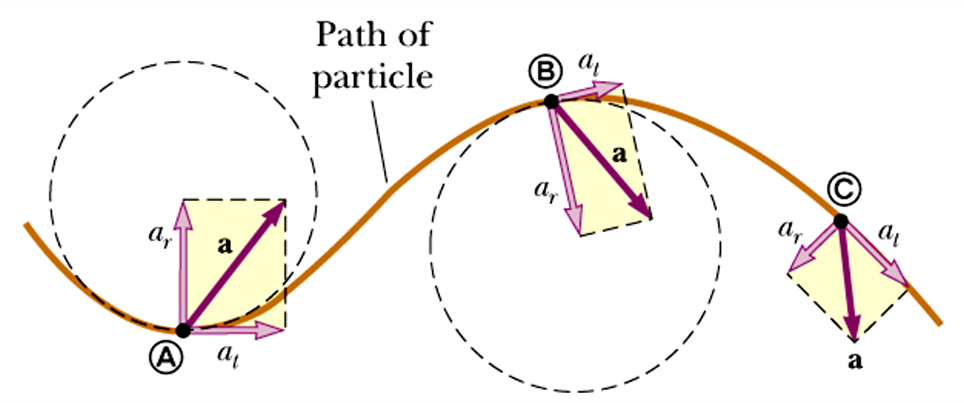
\includegraphics[width=0.7\linewidth]{images/particle path.png}
\end{center}
\begin{itemize}
    \item Computing tangential and radial components
    \begin{itemize}
        \item $\abs{a_t} = \abs{\mathbf{a} \cdot \hat{v}} = \frac{\abs{\mathbf{a\cdot v}}}{\abs{\mathbf{v}}}$
        \item $\mathbf{a}_t = \pm \abs{a_t}\hat{v}$
    \end{itemize}
    \item Tangential and radial components add up to the original acceleration: $\mathbf{a} = \mathbf{a}_r + \mathbf{a}_t$
    \begin{center}
        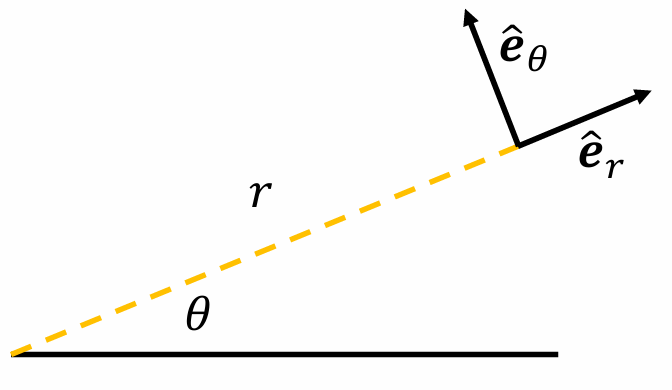
\includegraphics[width=0.5\linewidth]{images/kinematics polar coordinates.png}
    \end{center}
    \item Change of unit vectors along path: $\dv{\uvec{e}_r}{t} = \dv{\theta}{t} \uvec{e}_\theta$, $\dv{\uvec{e}_\theta}{t} = -\dv{\theta}{t} \uvec{e}_r$
    \item Velocity: $\vb{v} = \dv{\vb{r}}{t} = \dv{t}(r \uvec{e}_r) = \dv{r}{t}\uvec{e}_r + r\dv{\uvec{e}_r}{t} = \dv{r}{t}\uvec{e}_r + r\dv{\theta}{t}\uvec{e}_\theta$
    \item Acceleration: $\vb{a} = \dv{\vb{v}}{t} = \left[ \dv[2]{r}{t} - r \left( \dv{\theta}{t} \right)^2 \right] \uvec{e}_r + \left[ r \dv[2]{\theta}{t} + 2 \dv{r}{t}\dv{\theta}{t} \right] \uvec{e}_\theta$
    \item For constant radius: 
    \begin{itemize}
        \item $\vb{v} = r\dv{\theta}{t}\uvec{e}_\theta = v\uvec{e}_\theta = r\omega\uvec{e}_\theta$
        \item $\vb{a} = -r \left(\dv{\theta}{t} \right)^2 \uvec{e}_r + r\dv[2]{\theta}{t}\uvec{e}_\theta = a_r\uvec{e}_r + a_t\uvec{e}_\theta$, where $a_r = -r \left(\dv{\theta}{t}\right)^2 = -r\omega^2 \text{ and } a_t = r\dv[2]{\theta}{t} = \alpha$
    \end{itemize}
    \item Uniform circular motion $\rightarrow$ constant speed and angular velocity: $\dv{\omega}{t} = \dv[2]{\theta}{t} = 0 \text{ , } \dv{r}{t} = 0$. Also, $\vb{a} = a\uvec{e}_r \text{ where } a = -r\omega^2 = -\frac{v^2}{r}$ is a constant
    \item For non-uniform circular motion, there will be non-zero tangential acceleration where $\vb{a}_t = a_t\uvec{e}_\theta $ and $ a_t = \dv{v}{t}$
    \item 3D description: we introduce angular velocity vector $\vb{\omega(t)}$. If we put origin on rotation axis, we get compact formula $\dot{\vb{r}} = \vb{\omega}(t) \cross \vb{r}(t)$ and $\abs{\vb{\omega}(t) \cross \vb{r}(t)} = \abs{\vb{\omega}(t)}s$, where s is the shortest distance to the axis
\end{itemize}

\subsection{Relative Motion}
\begin{itemize}
    \item For non-rotating frame:
    \begin{center}
        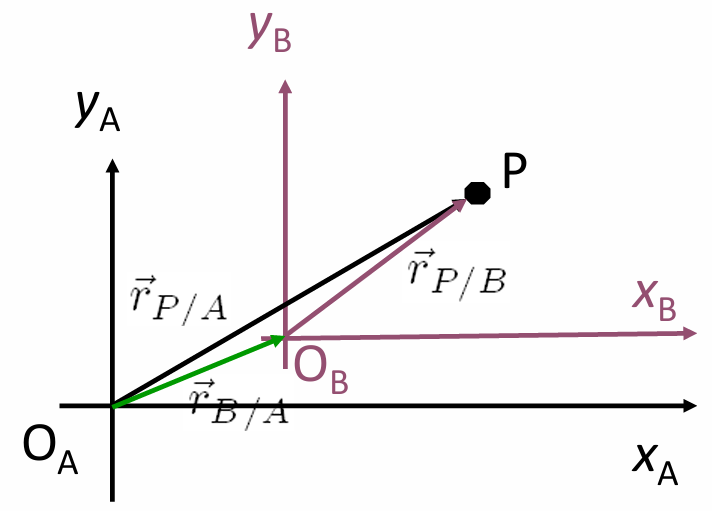
\includegraphics[width=0.5\linewidth]{images/non-rotating frame.png}
    \end{center}
    \item Converting frame of reference: $\vb{r}_{P/B} = \vb{r}_{P/A} - \vb{r}_{B/A}$
    \item Differentiate further to get: $\vb{v}_{P/B} = \vb{v}_{P/A} - \vb{v}_{B/A}$ and $\vb{a}_{P/B} = \vb{a}_{P/A} - \vb{a}_{B/A}$
    \item We also say that frame A is co-moving with particle 1 to indicate that particle 1's frame of reference is A
    \item Special case (velocity of B w.r.t A is constant): $\vb{r}_{P/B} = \vb{r}_{P/A} - \vb{v}_{B/A}t$, $\vb{v}_{P/B} = \vb{v}_{P/A} - \vb{v}_{B/A}$, $\vb{a}_{P/B} = \vb{a}_{P/A}$
    \item For rotating frames with constant angular velocity, consider frame B rotating w.r.t frame A:
    \begin{itemize}
        \item No translational motion
        \item Rotation axis passes through origin
        \item Angular velocity vector $\vb{\Omega}$ is constant
    \end{itemize}
    Then, we have $\vb{a}_{P/B} = \vb{a}_{P/A} + \vb{a}_{\text{centrifugal}} + \vb{a}_{\text{Coriolis}}$
    \item Centrifugal acceleration has direction outward from rotation axis and magnitude $s\Omega^2$, where $s$ is shortest distance from rotation axis
    \item Coriolis acceleration: $\vb{a}_{\text{Coriolis}} = -2\vb{\Omega} \cross \vb{v}_{P/B}$. Note that it is always perpendicular to $\vb{v}_{P/B}$ and is caused by rotating frame 
\end{itemize}

% ====================================================
%                      Chapter 2
% ====================================================

\section{2. Newtonian Physics}
\subsection{Newton's Laws}
\begin{itemize}
    \item Newton's first law, retconned: an inertial frame is defined as a reference frame where for all (point) masses, no forces implies $\vb{v}$ is constant and $\vb{a}$ = 0
    \item Newton's second law, retconned: the acceleration of a (point) mass in an inertial frame is proportional to the net force acting on it, $\vb{F}_{net} = m\vb{a}$
    \item Newton's third lad: $\vb{F}_{12} = -\vb{F}_{21}$
\end{itemize}

\subsection{Centre of Mass and Extended bodies}
\begin{itemize}
    \item Applying Newton's second law to extended bodies, we get $\vb{F}_{\text{net external}} = \dv{\vb{p}_{\text{total}}}{t} = m\vb{a}_{\text{CM}}$
    \item Formula for finding centre of mass: $\vb{r}_{\text{CM}} = \frac{\int\vb{r}dm}{m_{\text{total}}} = \frac{\int \vb{r} \rho(\vb{r})dV}{m_{\text{total}}} = \frac{\int \vb{r} \rho(\vb{r})dV}{\int \rho(\vb{r})dV}$
    \item Use $\sigma dA$ for mass per unit area, $\lambda dl$ for mass per unit length
    \item Centre of mass formula for 2 objects: $\vb{r}_{\text{CM}} = \frac{M\vb{R} + m\vb{r}}{M + m}$, where $\vb{r}^{\text{rel}} = \vb{r} - \vb{R}$
\end{itemize}

\subsection{More Applications}
\begin{itemize}
    \item When an object is about to lose contact, normal force $N = 0$
    \item Tension and normal force can act as a constraint force, preventing object from passing through a surface or allow an object to be at rest. Typically, tension and normal force equal to weight.
    \item Hooke's law: $F_s = -kx$
    \item Eg.
    \begin{center}
        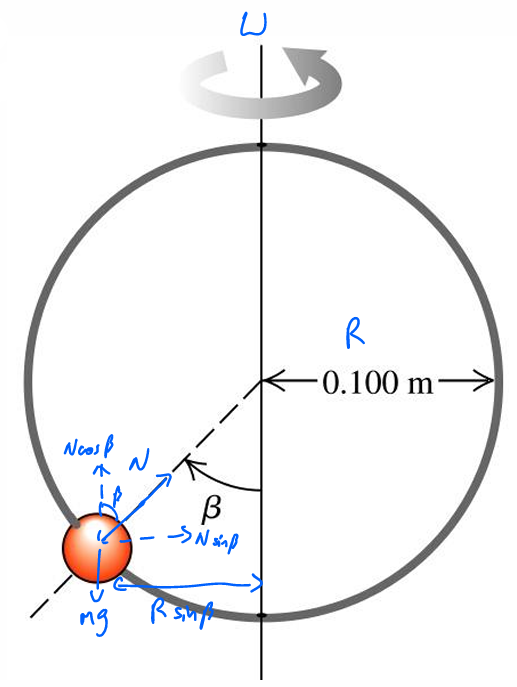
\includegraphics[width=0.3\linewidth]{images/bead on hoop.png}
    \end{center}
    Forces acting on the bead are: normal force and weight.\\ 
    y-direction: $N_y = mg$\\
    x-direction: $\text{centripetal force} = N_x$
    \item Static friction $f_s \leq \mu_sN$ opposes forces to prevent a stationary object from moving
    \item Kinetic friction $f_k = \mu_kN$ opposes the movement of a moving object, often slowing it down
    \item Generally, $\mu_k < \mu_s$
    \item For small objects at low speeds, $\vb{F} = -k\vb{v}$
    \item For large objects at high speeds, $\vb{F} = -D\abs{\vb{v}}\vb{v} = -D\abs{\vb{v}}^2 \uvec{v}$
    \item Terminal speed kinematics: $\dv{v}{t} = g - \frac{k}{m}v$, $v = (mg/k)\left(1-e^{-kt/m}\right)$
    \item Air drag at high speeds: $mg - Dv^2 = ma$, terminal speed $v_t = \sqrt{mg/D}$
    \item Newton's first and second laws only hold in inertial frames. If we consider frames that are accelerated, we can deal with the extra accelerated terms by introducing fictitious force $\vb{F}_{\text{fic}} = -m\vb{a}$ in the accelerated frame
    \item For rotating frames with angular velocity $\Omega$, introduce fictitious forces $\vb{F}_{\text{centrifugal}}$ with magnitude $ms\Omega^2$ directed outwards from rotation axis and $\vb{F}_{\text{Coriolis}} = -2m\Omega \cross \vb{v}_{P/B}$
\end{itemize}

% ====================================================
%                      Chapter 3
% ====================================================

\section{3. Energy}
\subsection{Energy and Work Done}
\begin{itemize}
    \item Work done $W = \int\vb{F}\cdot d\vb{x}$
    \item To compute the work done in a path, we compute the line integral of the path
    \item Eg.
    \begin{center}
        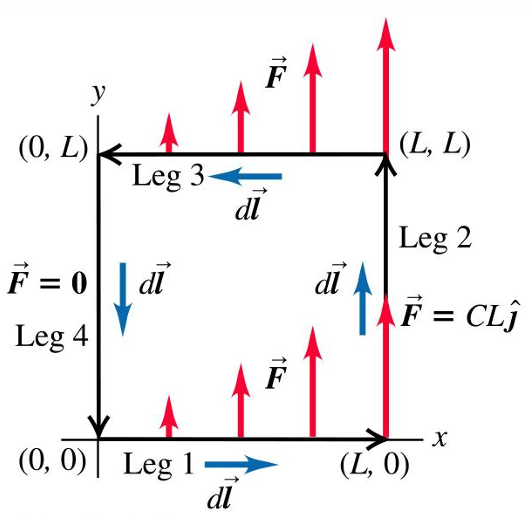
\includegraphics[width=0.5\linewidth]{images/line integral.png}
    \end{center}
    Given the force on an electron to be $\vb{F} = Cx\uvec{j}$ for some positive constant $C$, we have:
    \begin{itemize}
        \item $\int_{P_1}\vb{F}\cdot d\vb{x} = \int_{P_1}Cx\uvec{j} \cdot \uvec{i} \ dx = 0$
        \item $\int_{P_2}\vb{F}\cdot d\vb{x} = \int_{P_2} CL\uvec{j}\cdot \uvec{j} \ dy = CL^2$
        \item $\int_{P_3}\vb{F}\cdot d\vb{x} = 0$
        \item $\int_{P_4}\vb{F}\cdot d\vb{x} = \int_{P_4} C(0)\uvec{j} \cdot d\vb{x} = 0$
    \end{itemize}
    \item Work-Energy Theorem: work done = change in kinetic energy
    \item Power is energy per unit time and is denoted by $P = \vb{F} \cdot \dv{\vb{x}}{t} = \vb{F} \cdot \vb{v}$
    \item Similarly, $W = \int_P \vb{F} \cdot d\vb{x} = \int_{t_i}^{t_f} \vb{F} \cdot \dv{\vb{x}}{t} dt = \int_{t_i}^{t_f} P \ dt$
    \item Constraint forces generally act perpendicular to motion so they do no net work. Hence, we can ignore work done by constraint forces
\end{itemize}

\subsection{Conservation of Energy}
\begin{itemize}
    \item Conservative forces have these properties:
    \begin{itemize}
        \item Work done by $\vb{F}$ is path-independent
        \item Work done by $\vb{F}$ around any closed path is zero
        \item There exists scalar function $U$ such that $\vb{F} = -\nabla U$ (+ very mild assumptions)
    \end{itemize}
    \item Non-conservative forces include friction, resistive forces/drag and some electromagnetic effects
    \item Potential energy function $U(\vb{x}) = -\int_{\bf{O}}^{\vb{x}} \vb{F} \cdot d\vb{x}'$ for some origin point $\bf{O}$
    \item Potential energy property: $U(\vb{x}_2) - U(\vb{x}_1) = -\int_{\vb{x}_1}^{\vb{x}_2} \vb{F} \cdot d\vb{x}'$
    \item Potential energy of a spring is $U_{\text{spring}} = \frac{1}{2}kx^2$, where $x$ is displacement from "rest length" position
    \item Work-Energy, Extended Bodies Equation:
    \begin{center}
        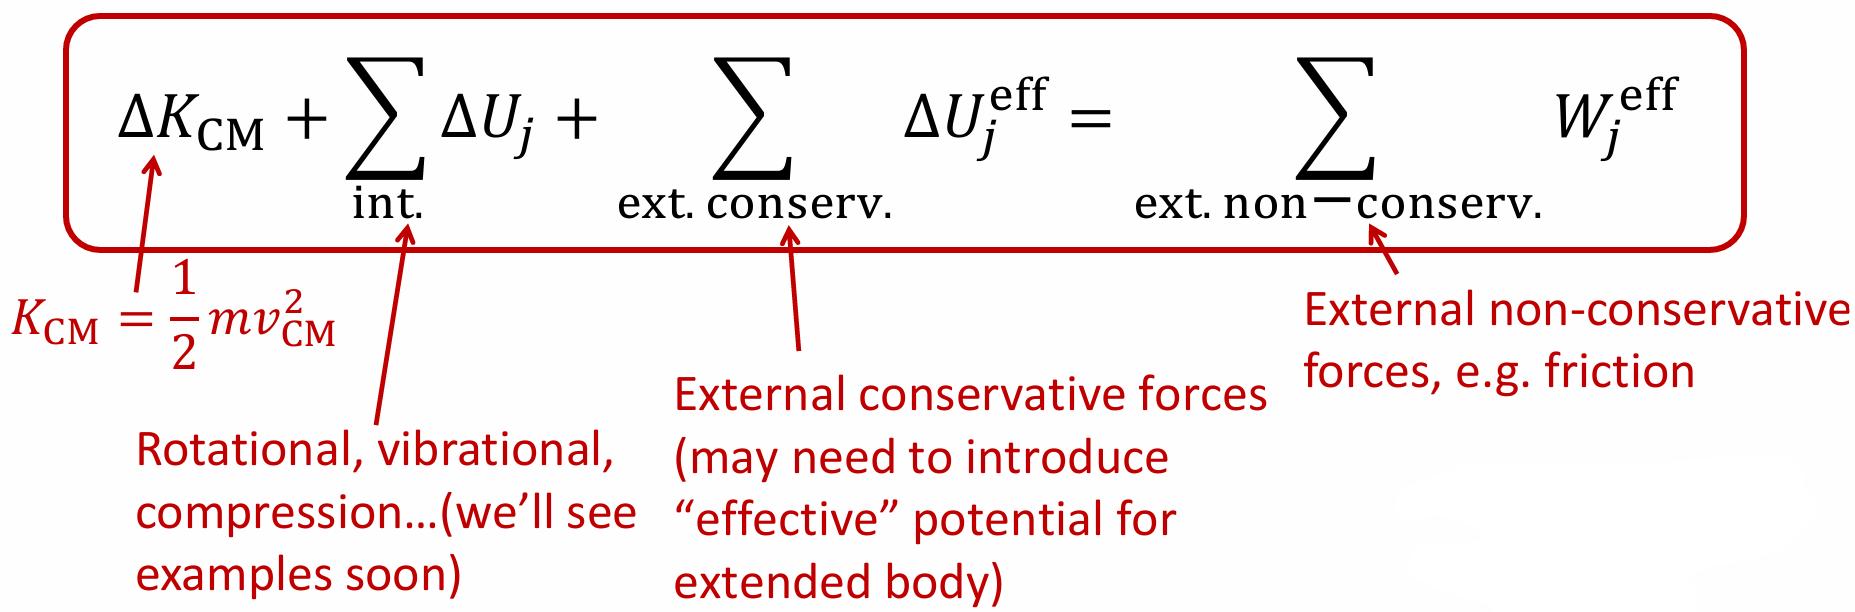
\includegraphics[width=0.9\linewidth]{images/work-energy, extended bodies.png}
    \end{center}
\end{itemize}

\subsection{Potentials}
\begin{itemize}
    \item Potential Energy Graph:
    \begin{center}
        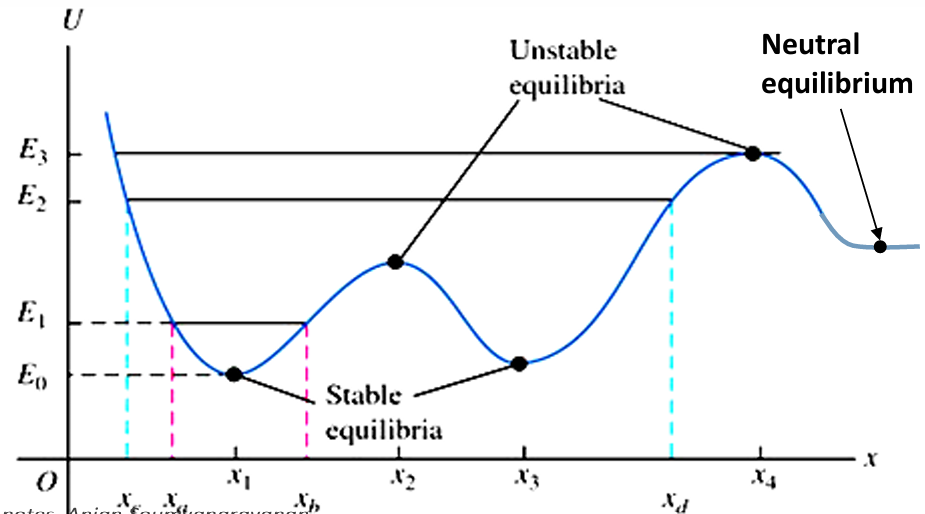
\includegraphics[width=0.9\linewidth]{images/potential energy graph.png}
    \end{center}
    \item Given a constant total energy $E$,
    \begin{itemize}
        \item For abstract $U(x)$, speed is $\abs{\dot{x}} = \sqrt{\frac{2(E-U)}{m}}$
        \item For gravitational $U = mgh$, speed is also $\abs{\vb{v}} = \sqrt{\frac{2(E-U)}{m}}$ 
        \item However, $\vb{v}$ is tangent to trajectory while $\abs{\dot{x}}$ is only its x-component, so generally $\abs{\vb{v}} \neq \abs{\dot{x}}$
    \end{itemize}
    \item Special case: equilibrium position; $F = 0$
    \begin{itemize}
        \item Stable equilibrium - particle "returns" to equilibrium position, though with oscillation
        \item Unstable equilibrium - particle runs away
        \item Neutral equilibrium - particle stays still
    \end{itemize}
    \item Simple harmonic motion formula can be generalized to $\ddot{q} = -\omega^2q$, where $q$ can be replaced with $\theta$ or $r$
    \item Note that $q$ is displacement of a coordinate from equilibrium, and is useful to substitute $q \coloneqq Q - Q^{\text{eq}}$
    \item Approximate harmonic motion uses Taylor expansion to obtain $\ddot{Q} \approx f'(Q^{\text{eq}})(Q - Q^{\text{eq}})$, or $\ddot{q} \approx f'(q^{\text{eq}})q$ for $q \coloneqq Q - Q^{\text{eq}}$
    \item For energy, as long as $U''(Q^{\text{eq}}) \neq 0$, we have $U(Q) \approx U(Q^{\text{eq}}) + \frac{U''(Q^{\text{eq}})}{2}(Q - Q^{\text{eq}})^2$
    \item By linearity, for more than 1 dimension, we can just add their potentials to study their behaviour. Doing so will give $U_{\text{total}}(\vb{r}) = -\int_{\text{origin}}^{\vb{r}} \vb{F}_{\text{total}} \cdot d\vb{r}$
    and $\vb{F}_{\text{total}} = - \nabla U_{\text{total}}$
\end{itemize}

% ====================================================
%                      Chapter 4
% ====================================================

\section{4. Momentum}
\subsection{Collisions}
\begin{itemize}
    \item Conservation of momentum (CoM) states that if net external force is zero, total momentum is constant, i.e. $\vb{p}_i = \vb{p}_f$
    \item We can also regroup the particles to write $\vb{p}_{\text{total}} = m_{\text{total}}\vb{v}_{\text{CM}}$
    \item In CM frame, total momentum is always zero if net external force is zero
    \item Impulse ($\Delta\vb{p}$):
    \begin{center}
        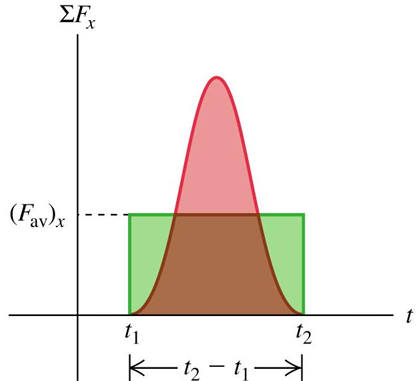
\includegraphics[width=0.5\linewidth]{images/impulse diagram.png}
    \end{center}
    Since $\vb{F}_{\text{net}} = \dv{\vb{p}}{t}$, we have $\Delta\vb{p} = \int_{t_i}^{t_f} \vb{F}_{\text{net}}\ dt$. We sometimes denote as $\vb{J}$
    \item Common classifications for collisions:
    \begin{itemize}
        \item Elastic collision: both momentum and KE conserved
        \item Inelastic collision: momentum conserved, KE not conserved
        \begin{itemize}
            \item Perfectly inelastic collision: particles "stick together", so they have the same final velocity
        \end{itemize}
    \end{itemize}
    \item Conservation of momentum: $m_1v_{1i} + m_2v_{2i} = m_1v_{1f} + m_2v_{2f}$
    \item Conservation of (kinetic) energy: $m_1v_{1i}^2 + m_2v_{2i}^2 = m_1v_{1f}^2 + m_2v_{2f}^2$
    \item For 1D elastic collisions, $v_{1f} = \left(\frac{m_1 - m_2}{m_1 + m_2}\right)v_{1i} + \left(\frac{2m_2}{m_1 + m_2}\right)v_{2i}$; $v_{2f} = \left(\frac{2m_1}{m_1 + m_2}\right)v_{1i} + \left(\frac{m_1 - m_2}{m_1 + m_2}\right)v_{2i}$
    \item For 1D perfectly inelastic collisions, $v_f = \frac{m_1v_{1i} + m_2v_{2i}}{m_1 + m_2} = v_{\text{CM}}$. This formula applies to higher dimensions as well (just replace $v$ with $\vb{v}$)
    \item For 2D collisions, apply conservation of momentum for $x$ and $y$ components
    \item For 3D collisions, find a plane such that the $z$-component of both particles' paths align, then solve it like the 2D collision case
\end{itemize}

\subsection{Variable Mass}
\begin{itemize}
    \item Rocket Science:
    \begin{center}
        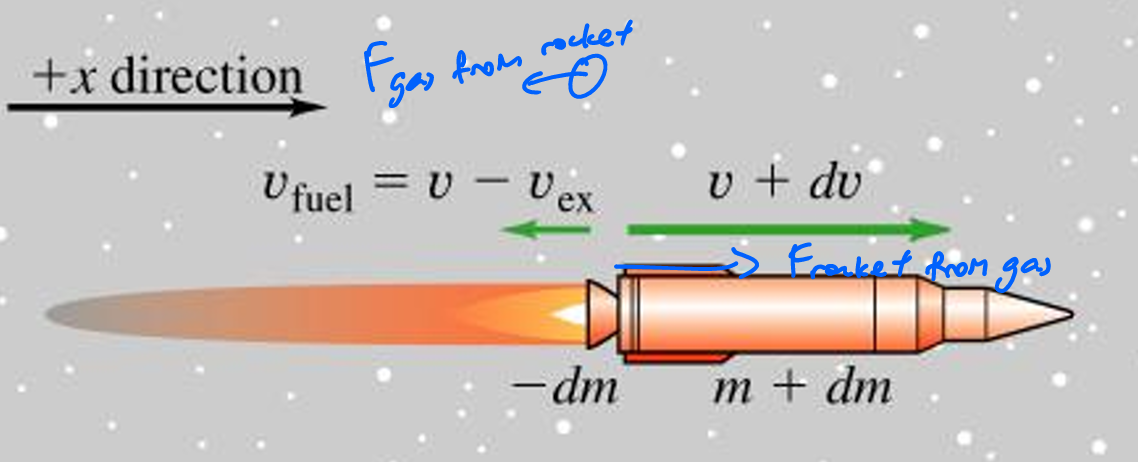
\includegraphics[width=0.7\linewidth]{images/rocket.png}
    \end{center}
    \item At time $t$,
    \begin{itemize}
        \item $m$: mass of rocket (note: this mass is changing)
        \item $v$: velocity of rocket (space frame)
    \end{itemize}
    \item At time $t + dt$,
    \begin{itemize}
        \item $m + dm$: mass of rocket ($dm < 0$)
        \item $v + dv$: velocity of rocket (space frame)
        \item $-dm$: mass of gas (note: $-dm > 0$)
        \item $v_{\text{fuel}}$: velocity of gas (space frame, so $v_{\text{fuel}} = v - u_{\text{ex}}$)
    \end{itemize} 
    Momentum at $t + dt$: $(m + dm)(v + dv) + (-dm)(v - u_{\text{ex}})$
    \\ Momentum at $t$: $mv$
    \\ No external forces so $p_{\text{total}}$ is constant, $\Delta p = 0$
    \\ After solving, we get: $v_f - v_i = u_{\text{ex}}\ln(m_i/m_f)$
    \\ note: in the process we get $dmdv \approx 0$ which is negligible
    \item If all exhaust exhausted at once, 
    \\Transform to frame where $v_i = 0$:
    \\ $m_fv_f = -(m_i-m_f)(v_f-u_{\text{ex}})$
    \\ Transform back: $v_f - v_i = \left(1 - \frac{m_f}{m_i}\right) u_{\text{ex}}$
    \item Example: Cart with Rain
    \\ At time $t + dt$: $p = (m + dm)(v + dt)$
    \\ At time $t$: $p = mv$
    \item Example: Leaky Cart
    \\ At time $t + dt$: $p = (m + dm)(v + dt) + (-dm)v$
    \\ At time $t$: $p = mv$
    \item If net external force is not zero, the "infinitesimal change" in total momentum is now $d\vb{p}_{\text{total}} = \vb{F_{\text{net external}}}dt$ instead of $0$
    \item Example: Falling Chain
    \begin{center}
        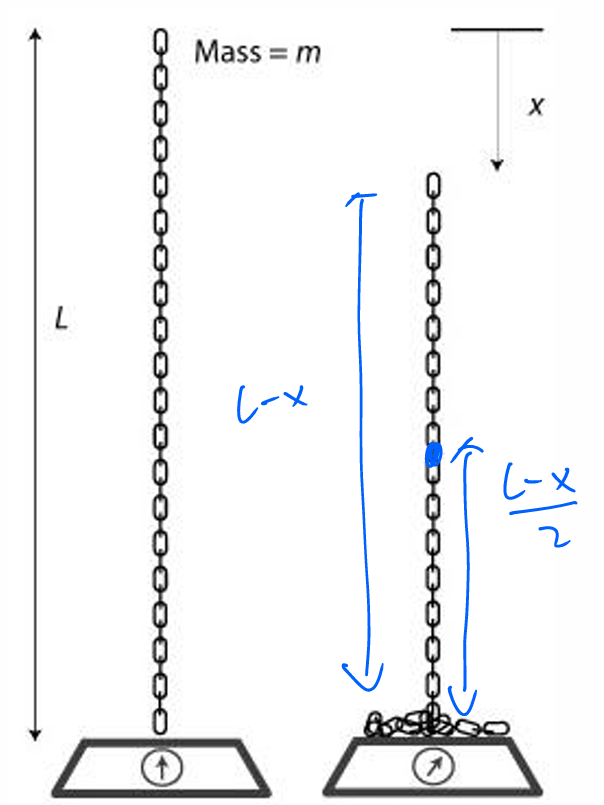
\includegraphics[width=0.4\linewidth]{images/falling chain.png}
    \end{center}
    Consider the bit that hits the scale
    \[
    \begin{aligned}
    dp &= F_{\text{stop}}dt \\
    (dm)\sqrt{2gx} - 0 &= F_{\text{stop}}dt \\
    F_{\text{stop}}dt &= \frac{2mgx}{L}
    \end{aligned}
    \]
    Find the reading on the scale \\
    $\hspace{70pt}\Rightarrow N = m_{\text{on scale}}g + F_{\text{stop}} = 3mgx/L$
\end{itemize}

% ====================================================
%                      Chapter 5
% ====================================================

\section{5. Rotational Mechanics}
\subsection{Rigid-Body Kinematics}
\begin{itemize}
    \item Often useful to consider positions of point masses relative to some point $\vb{r}_j^{\text{rel}}(t) = \vb{r}_j(t) - \vb{R}(t)$
    \item Rigid body is a set of point masses where distance between every pair of points must remain constant. Also, for every vector $\vb{\gamma}(t)$ of constant magnitude, $\vb{\dot{\gamma}} \perp \vb{\gamma}$
    \item For relative velocities between points at constant distance: $\vb{\dot{r}}_j^{\text{rel}}(t) \perp \vb{r}_j^{\text{rel}}(t)$
    \item Rigid body motion: $\vb{\dot{r}}_j^{\text{rel}}(t) = \vb{\omega}^{\text{rel}}(t) \cross \vb{r}_j^{\text{rel}}(t)$
    \item If we have relative instantaneous rotation: $\vb{\dot{r}}_j(t) = \vb{\dot{R}}(t) + \vb{\omega}^{\text{rel}}(t) \cross \vb{r}_j^{\text{rel}}(t)$
    \item Interpretation: each point's instantaneous velocity splits into instantaneous velocity of chosen point and instantaneous pure rotation about chosen point
    \begin{center}
        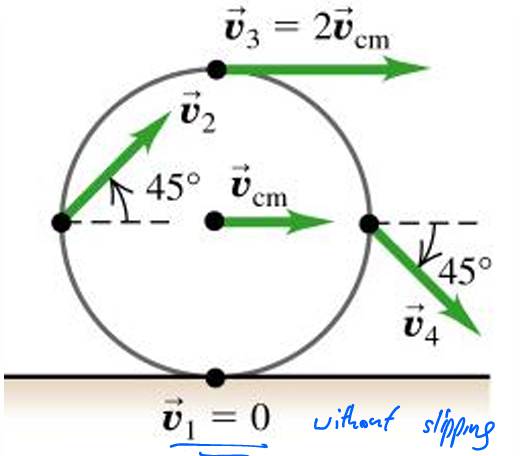
\includegraphics[width=0.5\linewidth]{images/rolling without slipping.png}
    \end{center}
    \item No slipping condition between two objects means that the contact points are stationary w.r.t. each other
    \item So for rolling without slipping, $s = R\theta$
    \begin{itemize}
        \item $v_{\text{centre}} = R\omega$
        \item $a_{\text{centre}} = R\alpha$, where $\alpha = \dv{\omega}{t}$ is angular acceleration
    \end{itemize}
    \item Since bottom-most point is stationary relative to surface, there is static friction but not kinetic friction, and static friction does no net work so it doesn't affect work-energy theorem
    \item For rolling in general, we may have $V_{\text{centre}} \neq R\omega$. So, it has kinetic friction instead of static friction and contact points of object and surface are not stationary w.r.t. each other
\end{itemize}

\subsection{Inertia and Energy}
\begin{itemize}
    \item (scalar) Moment of inertia, $I = \sum_j m_j s_j^2$
    \item Kinetic energy, $K_{\text{total}} = \frac{1}{2}I\omega^2$
    \item Moment of inertia depends only on rotation axis and object's current distribution of masses
    \item Moments of inertia can add up, e.g. $I_{\text{combined}} = I_1 + I_2$
    \item For "continuous" bodies with density $\rho$ (can vary over body), $I = \int \rho s^2 \ dV$. Use $\sigma \ dA$ or $\lambda \ dL$ instead for 2D or 1D respectively
    \item Example: Uniform Thin Rod
    \begin{center}
        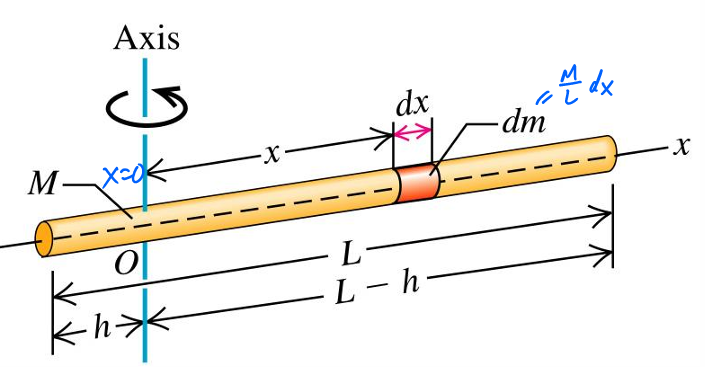
\includegraphics[width=0.7\linewidth]{images/uniform thin rod.png}
    \end{center}
    \[
    \begin{aligned}
        I &= \int_0^{L - h} \frac{M}{L}x^2 \ dx + \int_0^h \frac{M}{L} (-x)^2 \ dx \\
        &= \frac{M}{L} \int_{-h}^{L - h} x^2 \ dx \\
        &= \frac{M}{3L}(L^3 - 3L^2h + 3Lh^2)
    \end{aligned}
    \]
    \item Moment of inertia for common shapes:
    \begin{center}
        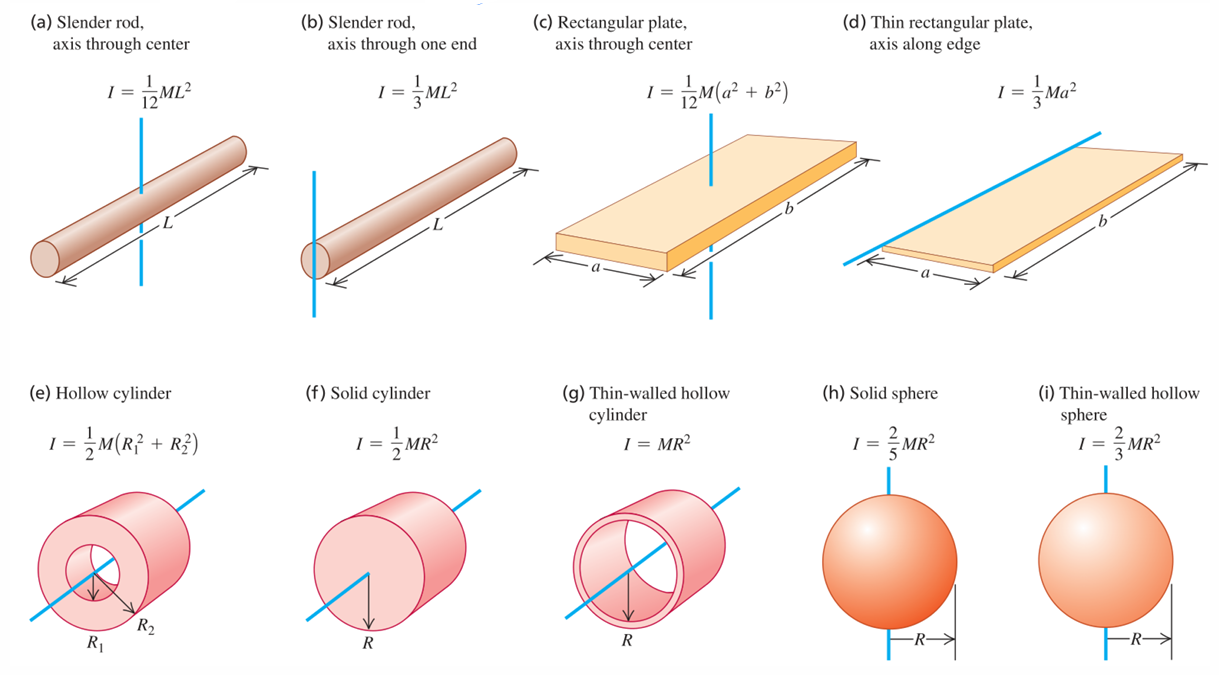
\includegraphics[width=1\linewidth]{images/inertia for common shapes.png}
    \end{center}
    \item Parallel-Axis Theorem: \\
    Given a rotation axis, moment of inertia $I$ about the axis satisfies
    \[
    \begin{aligned}
        I = m_{\text{total}}s_{\text{CM}}^2 + I_{\text{CM}}
    \end{aligned}
    \]
    \begin{itemize}
        \item $s_{\text{CM}}$ is CM distance from axis (perpendicular distance between the axes)
        \item $I_{\text{CM}}$ is MOI about the parallel axis that passes through CM
    \end{itemize}
    \item  Perpendicular-Axis Theorem:
    \begin{itemize}
        \item Given a 2D body, and 
        \item Any 2 perpendicular axes in the plane of the body, with corresponding moments of inertia $I_x$, $I_y$, intersecting at a point $P$,
        \item Moment of inertia $I_z$ about axis through $P$, perpendicular to plane of body, will be
    \end{itemize}
    \[
    \begin{aligned}
        I_z = I_x + I_y
    \end{aligned}
    \]
    \hspace{9pt} note: it doesn't work on non-2D body
    \item Important property: $\sum_j m_j \vb{r}_{j}^{\text{rel}} = 0$, i.e. "mass-weighted sum" of relative positions is zero
    \item Kinetic Energy Decomposition:
    \begin{itemize}
        \item $K_{\text{CM}} = \frac{1}{2}m_{\text{total}}\abs{\vb{\dot{R}}_{\text{CM}}}^2$
        \item $K_{\text{int}} = \frac{1}{2} \sum_j m_j \abs{\vb{\dot{r}}_j^{\text{rel}}}^2$
    \end{itemize}
    \item \bf{Warning}: only works for $R_{\text{CM}}$ (needs $\sum_j m_j \vb{r}_{j}^{\text{rel}} = 0$ trick)
    \item Kinematic Energy Decomposition (Rigid Body):
    \begin{itemize}
        \item $K_{\text{int}} = \frac{1}{2}\sum_j m_j \abs{\vb{\dot{r}}_j^{\text{rel}}}^2 = \frac{1}{2}\sum_j m_j \abs{\vb{\omega}^{\text{rel}} \cross \vb{r}_j^{\text{rel}}}^2 = \frac{1}{2} I_{\text{CM}}(\omega^{\text{rel}})^2$
        \item where $I_{\text{CM}} = \sum_j m_j \abs{s_j^{\text{rel}}}^2$ is a MOI about an axis through CM
    \end{itemize}
    \item Example: Hollow vs Solid Cylinder
    \begin{center}
        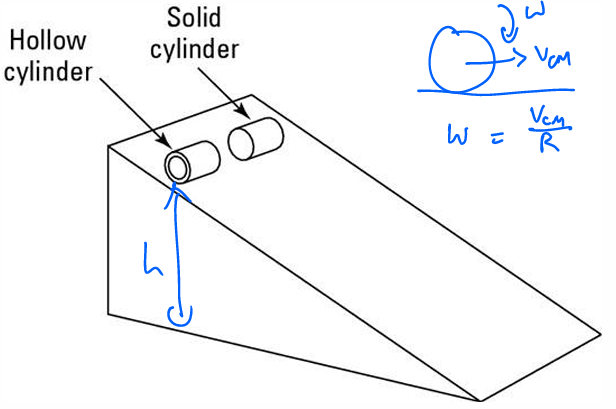
\includegraphics[width=0.7\linewidth]{images/hollow vs solid cylinder.png}
    \end{center}
    Assume no slipping, static friction does no net work, so energy is conserved.
    \[
    \begin{aligned}
        mgh &= K_{\text{total}} \\
        &= \frac{1}{2} mv_{\text{CM}}^2 + \frac{1}{2} I_{\text{CM}} \omega^2 \\
        &= \frac{1}{2} \left(m + \frac{I_{\text{CM}}}{R^2}\right) v_{\text{CM}}^2 \\
        v_{\text{CM}}^2 &= \frac{2gh}{1 + \frac{I_{\text{CM}}}{mR^2}} \\
    \end{aligned}
    \]
    Let $k = \frac{I_{\text{CM}}}{mR^2}$, \hspace{3pt}
    $v_{\text{CM}} \uparrow$ if $k \downarrow$. \\
    \vspace{3pt} Given both have same $R$, hollow cylinder has larger $k$ so it is slower than solid cylinder.
\end{itemize}

\subsection{Angular Momentum}
\begin{itemize}
    \item Angular Momentum, $\vb{L} = \vb{r} \cross \vb{p} = m\vb{r} \cross \vb{v} = m\vb{r} \cross \vb{\dot{r}}$
    \item For 2D motion, $\vb{L} = L^z\uvec{k}$
    
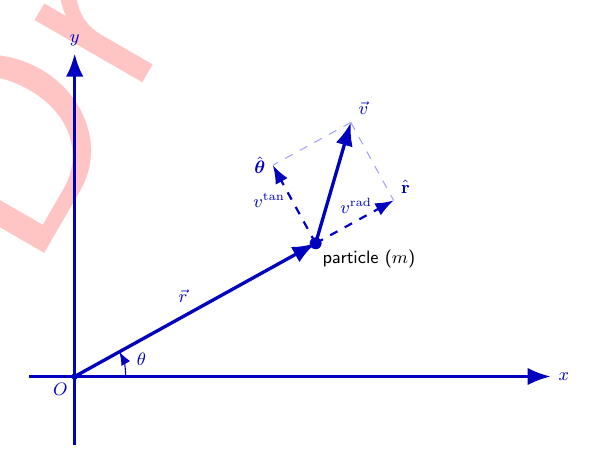
\begin{tikzpicture}[
  scale=0.72,
  transform shape,
  >=Latex,
  axis/.style={->,blue!75!black,very thick},
  vector/.style={->,blue!75!black,very thick},
  component/.style={->,blue!75!black,thick,dashed},
  guide/.style={blue!35,thin,dashed},
  every node/.style={font=\small}
]
  % Axes
  \coordinate (O) at (0,0);
  \coordinate (Xaxis) at (8.4,0);
  \draw[axis] (-0.8,0) -- (8.4,0) node[right] {$x$};
  \draw[axis] (0,-1.2) -- (0,5.7) node[above] {$y$};
  \fill[blue!75!black] (O) circle (1.6pt) node[below left] {$O$};

  % Position and polar angle
  \coordinate (P) at (4.25,2.35);
  \draw[vector] (O) -- (P) node[midway,above left] {$\vec r$};
  \pic[draw,blue!75!black,->,"$\theta$",angle radius=0.9cm,angle eccentricity=1.35]
    {angle = Xaxis--O--P};

  % Perpendicular radial and tangential velocity components
  \coordinate (Rdir) at ($(P)+(2.15,1.18)$);
  \coordinate (Tdir) at ($(P)+(-1.18,2.15)$);
  \coordinate (Rcomp) at ($(P)!0.64!(Rdir)$);
  \coordinate (Tcomp) at ($(P)!0.64!(Tdir)$);
  \draw[component] (P) -- (Rcomp) node[above right] {$\hat{\mathbf r}$};
  \draw[component] (P) -- (Tcomp) node[left] {$\hat{\boldsymbol\theta}$};
  \node[blue!75!black,above] at ($(P)!0.52!(Rcomp)$) {$v^{\mathrm{rad}}$};
  \node[blue!75!black,left] at ($(P)!0.55!(Tcomp)$) {$v^{\mathrm{tan}}$};

  % Exact vector sum: V-P=(Rcomp-P)+(Tcomp-P)
  \coordinate (V) at ($(Rcomp)+(Tcomp)-(P)$);
  \draw[vector] (P) -- (V) node[above right] {$\vec v$};
  \draw[guide] (V) -- (Rcomp);
  \draw[guide] (V) -- (Tcomp);
  \fill[blue!75!black] (P) circle (3pt) node[below right,black] {particle ($m$)};
\end{tikzpicture}
    
    \begin{itemize}
        \item $\vb{r} \cross \vb{v} = v^{\tan}s \uvec{k}$, where $v^{\tan} = \dot{\theta}s$ is tangential velocity component, and $s$ is distance from origin
        \item Conclusion: $L^z = ms^2\dot{\theta}$
    \end{itemize}    
    \item Consider 3D momentum:
    \begin{center}
        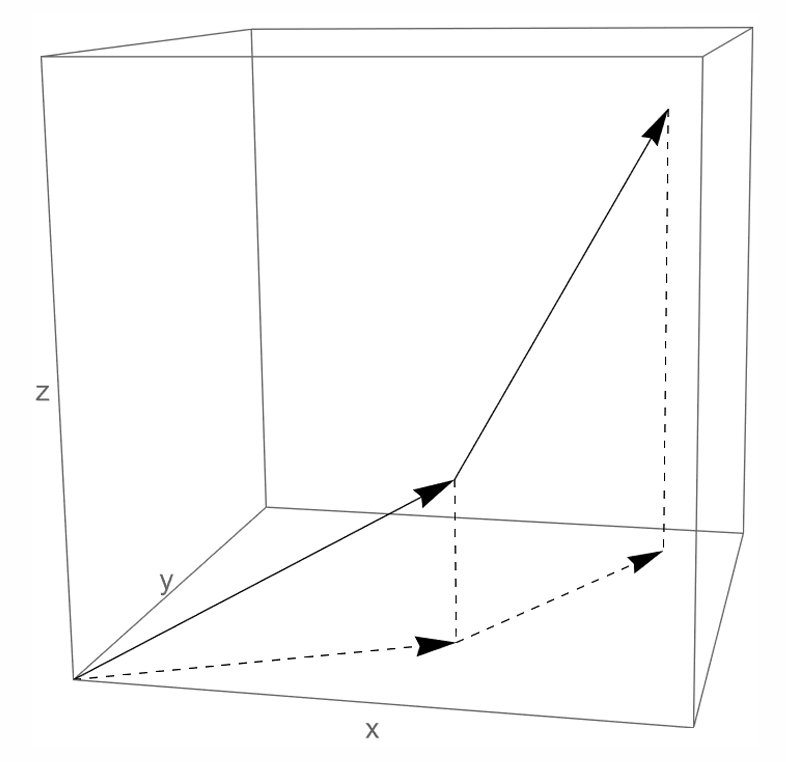
\includegraphics[width=0.5\linewidth]{images/3d angular momentum.png}
    \end{center}
    \item We can view it from the top to get $L^z \uvec{k} = m\vb{r}_{\text{proj}} \cross \vb{v}_{\text{proj}}$
    \item We have the same formula for 3D, $L^z = ms^2\dot{\theta}$, but $s = \abs{\vb{r}_{\text{proj}}} \neq \abs{\vb{r}}$
    \item For extended bodies, we have $L_{\text{total}}^z = \underset{j}{\sum} m_j s_j^2 \dot{\theta}_j$
    \item If we focus on pure rotation about chosen z-axis $\vb{\omega} = \omega^z \uvec{k}$, then all particles have same value $\dot{\theta}_j = \omega^z$
    \item Hence, we have $L_{\text{total}}^z = I\omega^z$ and $L_{\text{total}} = I\omega$ (implicitly only taking z-component)
    \item Torque, $\vb{\tau}^{\text{net external}} = \dv{\vb{L}_{\text{total}}}{t} = \underset{j}{\sum}\vb{r}_j \cross \vb{F}_j^{\text{net external}}$
    \item Taking z-component of torque, $\tau^z \uvec{k} = \vb{r}_{\text{proj}} \cross \vb{F}_{\text{proj}}$, where $\vb{r}_{\text{proj}} \perp \vb{F}_{\text{proj}}$
    \item If everyting is stationary, i.e. velocities are zero, $\vb{F}^{\text{net external}} = \dv{\vb{p}_{\text{total}}}{t} = 0$ and $\vb{\tau}^{\text{net external}} = \dv{\vb{L}_{\text{total}}}{t} = 0$
    \item Example: Force and Torque Equilibrium
    \begin{center}
        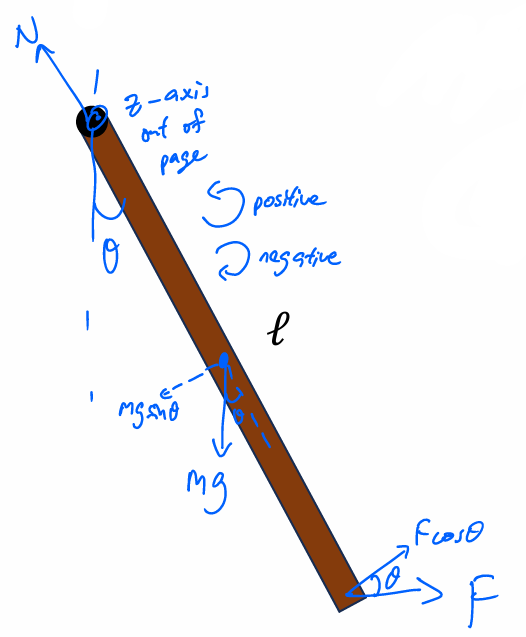
\includegraphics[width=0.4\linewidth]{images/torque on rod.png}
    \end{center}
    \[
    \begin{aligned}
        \tau^{\text{net}} &= -mg\sin\theta \frac{l}{2} + F\cos\theta = 0 \\
        \Rightarrow F\cos\theta &= \frac{1}{2}mg\sin\theta \\
        \theta &= \tanh\left( \frac{2F}{mg} \right)
    \end{aligned}
    \]
    Now, consider the forces in equlibrium,
    \[
    \begin{aligned}
        N_{\text{hor}} &= F \\
        N_{\text{vert}} &= mg
    \end{aligned}
    \]
    \item When torque is zero, $\vb{L}_{\text{total}} = 0$, angular momentum is conserved**
    \item Classic Example: Figure Skating \\
    Assume frictionless ice, when the skater pull back her arms, her speed increases. KE is not constant here. \\
    By CoAM, 
    \[
    \begin{aligned}
        I_i\omega_i &= I_f\omega_f \\
        \omega_f &= \frac{I_i}{I_f}\omega_i
    \end{aligned}
    \]
    Compare the initial and final kinetic energy,
    \[
    \begin{aligned}
        K_i &= \frac{1}{2}I_i\omega_i^2 \\
        K_f &= \frac{1}{2}I_f\omega_f^2 \\
        &= \frac{1}{2}\left( \frac{I_i}{I_f}\omega_i \right)^2 \\
        &= \frac{I_i^2}{2I_f}\omega_i^2
    \end{aligned}
    \]
    \item Angular Momentum Decomposition: \\
    \begin{center}
        $\vb{L}_{\text{total}} = \vb{L}_{\text{CM}} + \vb{L}_{\text{int}}$,
    \end{center} where
    \begin{itemize}
        \item $\vb{L}_{\text{CM}} = \vb{R}_{\text{CM}} \cross m_{\text{total}}\vb{\dot{R}}_{\text{CM}}$ ("Centre of mass angular momentum")
        \item $\vb{L}_{\text{int}} = \sum_j \vb{r}_j^{\text{rel}} \cross m_j\vb{\dot{r}}_j^{\text{rel}}$ ("Internal angular momentum")
    \end{itemize}
    \item Angular Momentum Decomposition (Rigid Body): $\vb{L}_{\text{int}} = I^{\text{mat}}\vb{\omega}^{\text{rel}}$, where matrix $I^{\text{mat}}$ (also called "moment of inertia tensor") is determined by body's current "geometry"
    \item We can handle $\vb{L}_{\text{int}}$ using scalar MOI for 2 cases:
    \begin{enumerate}
        \item One-Component Focus: Set z-axis through CM, parallel to $\vb{\omega}^{\text{rel}}$, focus on $L_{\text{int}}^z$. Then, we have $\vb{\omega}^{\text{rel}} = \omega^{\text{rel}} \uvec{k}$ and $L_{\text{int}}^z = I_{\text{CM}}\omega^{\text{rel}}$
        \item Symmetry: When object has "good" symmetry about CM, it simplifies to $\vb{L}_{\text{int}} = I_{\text{CM}}\vb{\omega}^{\text{rel}}$, where $\vb{L}_{\text{int}} \parallel \vb{\omega}^{\text{rel}}$, and $\vb{\omega}^{\text{rel}}$ is eigenvector of $I^{\text{mat}}$
    \end{enumerate}
    \item Example: Horizontal Rolling-Without Slipping
    \begin{center}
        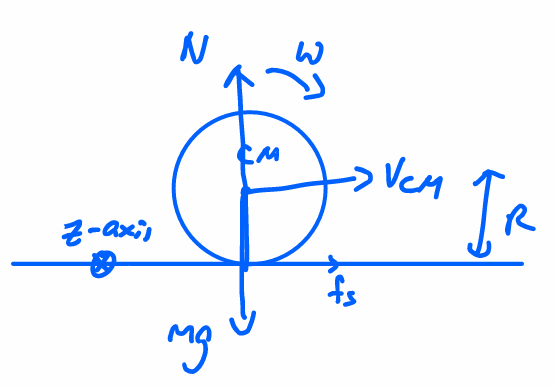
\includegraphics[width=0.5\linewidth]{images/rolling without slipping - torque.png}
    \end{center}
    Consider forces $N$ and $f_s$,
    \[
    \begin{aligned}
        N &= mg \\
        f_s &= ma_{\text{CM}}
    \end{aligned}
    \]
    Since $f_s$ contribution to torque is zero and contribution from $N$ and $mg$ cancel, $\tau_{\text{net}} = 0$,
    \[
    \begin{aligned}
        \tau_{\text{net}} &= \dv{L_{\text{total}}}{t} \\
        &= \dv{t}(L_{\text{CM}} + L_{\text{int}}) \\
        &= \dv{t}(mR^2\omega + I_{\text{CM}}\omega) \\
        &= (mR^2 + I_{\text{CM}})\dv{\omega}{t}
    \end{aligned}
    \]
    Since $mR^2 + I_{\text{CM}} \neq 0$, we have $\dv{\omega}{t} = 0$ \\
    $\omega$ is constant $\Rightarrow \abs{\vb{v}_{\text{CM}}}$ is constant $\Rightarrow f_s = 0$
    \item Example: Rotating Paddle
    \begin{center}
        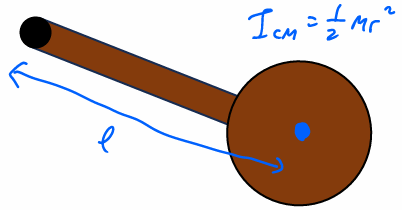
\includegraphics[width=0.5\linewidth]{images/rotating paddle.png}
    \end{center}
    \begin{itemize}
        \item Method 1: parallel axis theorem, $I = ml^2 + \frac{1}{2}mr^2$ about this axis, so $L = I\omega = \left( ml^2 + \frac{1}{2}mr^2 \right) \omega$
        \item Method 2: $L = L_{\text{CM}} + L_{\text{int}} = ml^2\omega + I_{\text{CM}}\omega^{\text{rel}} = \left( ml^2 + \frac{1}{2}mr^2 \right) \omega$
    \end{itemize}
    \item Example: Point and Stick
    \begin{center}
        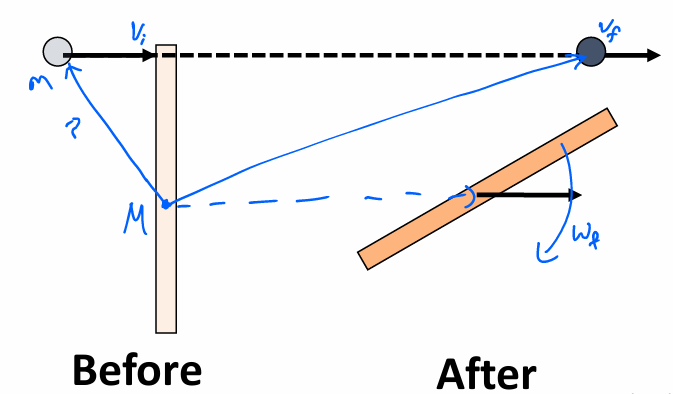
\includegraphics[width=0.6\linewidth]{images/point and stick.png}
    \end{center}
    Pick origin to be original CM position of stick, pick z-axis to be pointing into the page, then angular momentum about that axis are:
    \begin{itemize}
        \item Point mass: $\frac{l}{2}mv_i \rightarrow \frac{l}{2}mv_f$
        \item Stick: $0 \rightarrow L_{\text{CM}} + I\omega_f = I\omega_f$        
    \end{itemize}
    Putting it together:
    \begin{itemize}
        \item Conservation of (linear) momentum, horizontal: $mv_i = mv_f + MV_f$
        \item Conservation of angular momentum: $\frac{l}{2}mv_i = \frac{l}{2}mv_f + I\omega_f$
        \item Conservation of KE: $mv_i^2 = mv_f^2 + MV_f^2 + I\omega_f^2$
    \end{itemize}
    Solve them to get
    \[
    \begin{aligned}
        v_f &= \frac{4m - M}{4m + M}v_i \\
        V_f &= \frac{2m}{4m + M}v_I \\
        \omega_f &= \frac{12m}{4m + M}\left(\frac{v_i}{l}\right)
    \end{aligned}
    \]
\end{itemize}

\subsection{Torque}
\begin{itemize}
    \item For pure rotation of a rigid body, $\tau_{\text{net external}}^z = I \dv{\omega^z}{t} = I\alpha$, where $\alpha$ is the angular acceleration
    \item Example: Swinging Trapdoor
    \begin{center}
        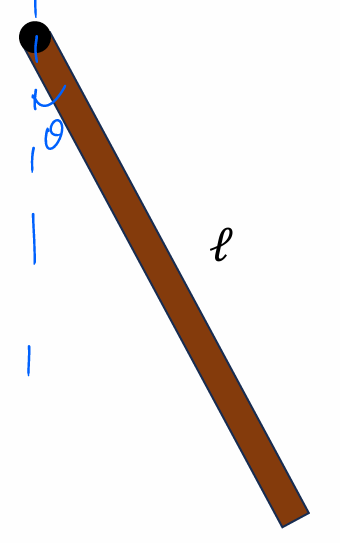
\includegraphics[width=0.3\linewidth]{images/swinging trapdoor.png}
    \end{center}
    \[
    \begin{aligned}
        \tau_{\text{net}} &= mg\frac{l}{2}\sin\theta \\
        \tau_{\text{net}} &= I\alpha \\
        \Rightarrow mg\frac{l}{2}\sin\theta &= \frac{ml^3}{3}\alpha \\
        \ddot{\theta} &= -\alpha \\
        &= -\frac{3g}{2l}\sin\theta\\
        &\approx -\frac{3g}{2l}\theta \\
        \omega^2 &= \frac{3g}{2l}
    \end{aligned}
    \]
    \item For uniform gravity $\vb{g}$ on extended object, total gravitational torque is the same as though it acts at CM
    \begin{center}
        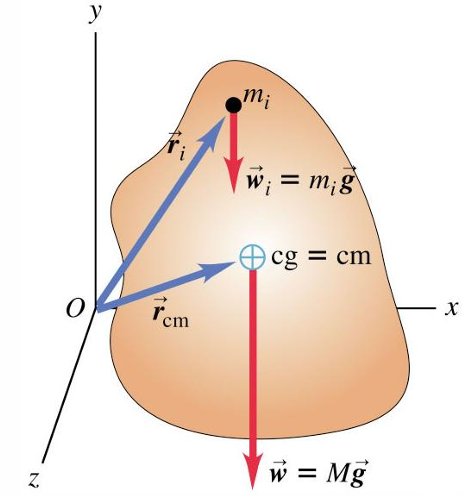
\includegraphics[width=0.3\linewidth]{images/uniform gravity.png}
    \end{center}
    $\vb{\tau}_{\text{total grav}} = \sum_j \vb{r}_j \cross m_j\vb{g} = \left(\sum_j m_j\vb{r}_j\right) \cross \vb{g} = m_{\text{total}}\vb{r}_{\text{CM}} \cross \vb{g} = \vb{r}_{\text{CM}} \cross (m_{\text{total}}\vb{g})$
    \item Tension acts on the point(s) where rope "leaves" pulley/spool/etc
    \item Example: Tension on Yo-Yo / Spool
    \begin{center}
        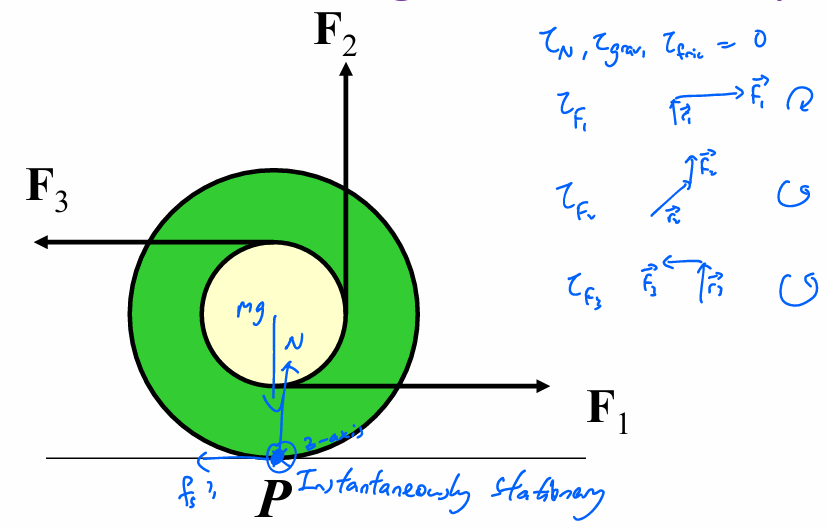
\includegraphics[width=0.7\linewidth]{images/yoyo.png}
    \end{center}
    \begin{center}
        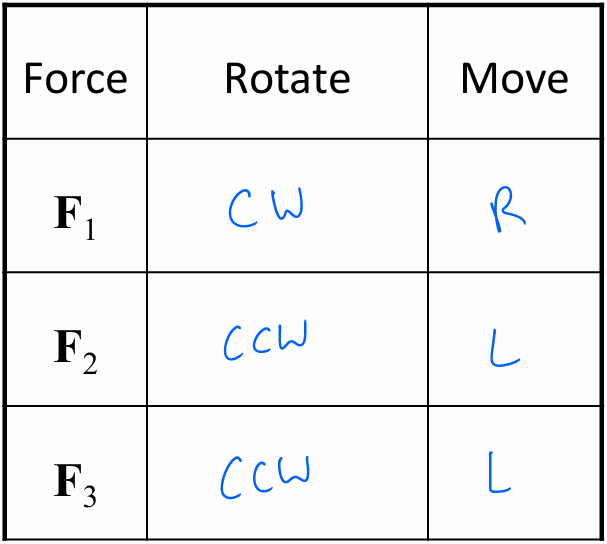
\includegraphics[width=0.4\linewidth]{images/forces on yoyo.png}
    \end{center}
    \item Example: Ball Rolling Downhill \\
    Pick z-axis along the CM 
    \begin{center}
        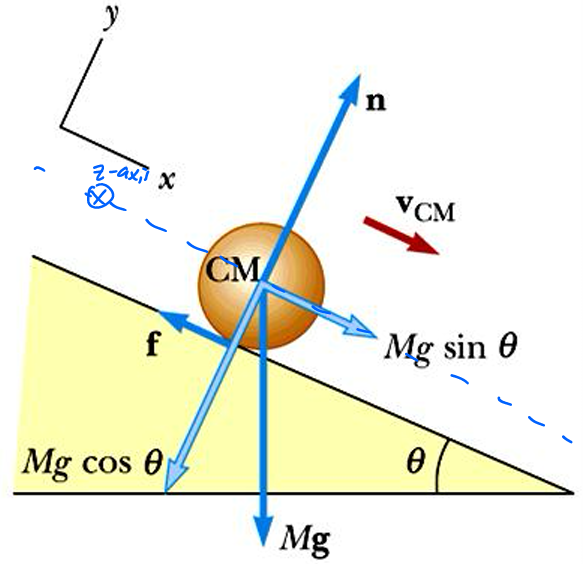
\includegraphics[width=0.4\linewidth]{images/ball rolling downhill.png}
    \end{center}
    By Newton's second law,
    \[
    \begin{aligned}
        n - Mg\cos\theta &= 0 \\
        Mg\sin\theta - f &= Ma_{\text{CM}}
    \end{aligned}
    \]
    Assume no-slip, $a_{\text{CM}} = R\alpha$ \\
    Rotation: 
    \[
    \begin{aligned}
        L_{\text{total}} &= L_{\text{CM}} + L_{\text{int}} = I_{\text{CM}}\omega \\
        \tau_{\text{net}} &= \tau_{\text{normal}} + \tau_{\text{grav}} + \tau_{\text{fric}} \text{ ($\tau_{\text{normal}}$ and $\tau_{\text{grav}\perp}$ cancel off)} \\
        &= \tau_{\text{grav //}} + \tau_{\text{fric}} \\
        &= Rf \\
        \tau_{\text{net}} &= \dv{L_{\text{total}}}{t} \\
        \Rightarrow Rf &= I_{\text{CM}}\alpha = I_{\text{CM}}\frac{a_{\text{CM}}}{R} \\
        \Rightarrow f &= \frac{I_{\text{CM}}}{R^2}a_{\text{CM}} \\
        &= \frac{2}{7}Mg\sin\theta
    \end{aligned}
    \]
    Substitute $f$ to get
    \[
    \begin{aligned}
        Mg\sin\theta - \frac{I_{\text{CM}}}{R^2}a_{\text{CM}} &= Ma_{\text{CM}} \\
        a_{\text{CM}} &= \frac{Mg\sin\theta}{M + \frac{I_{\text{CM}}}{R^2}}
    \end{aligned}
    \]
    Alternatively, pick z-axis at the point where the ball contact the slope
    \begin{center}
        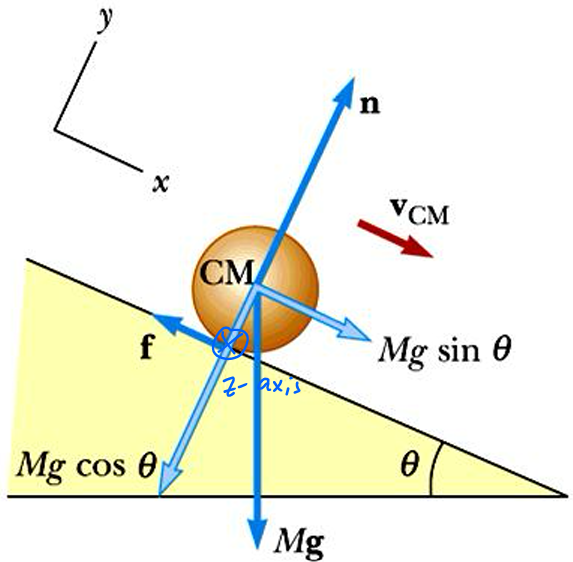
\includegraphics[width=0.4\linewidth]{images/ball rolling downhill 2.png}
    \end{center}
    At the point chosen, $\tau_{\text{fric}} = 0$, $\tau_{\text{normal}} = 0$ and $\tau_{\text{grav}\perp} = 0$
    \[
    \begin{aligned}
        \tau_{\text{net}} &= \tau_{\text{grav //}} = RMg\sin\theta \\
        L_{\text{total}} &= L_{\text{CM}} + L_{\text{int}} = \left( RM + \frac{I_{\text{CM}}}{R} \right)v_{\text{CM}} \\
        \tau_{\text{net}} &= \dv{L_{\text{total}}}{t} \\
        \Rightarrow RMg\sin\theta &= \left( RM + \frac{I_{\text{CM}}}{R} \right)v_{\text{CM}} \\
        a_{\text{CM}} &= \frac{Mg\sin\theta}{M + \frac{I_{\text{CM}}}{R^2}} \\
        &= \frac{5}{7}g\sin\theta
    \end{aligned}
    \]
    \item Rolling with slipping: $V_{\text{CM}} > R\omega$
    \begin{center}
        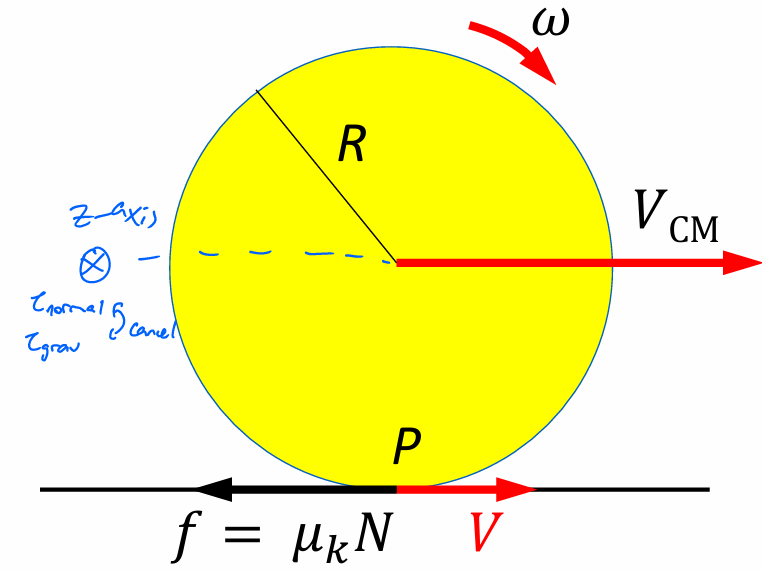
\includegraphics[width=0.5\linewidth]{images/rolling with slipping.png}
    \end{center}
    If CM at centre:
    \[
    \begin{aligned}
        M\dv{V_{\text{CM}}}{t} &= -f \\
        \tau_{\text{net}} &= \dv{L_{\text{total}}}{t} \\
        fR &= \dv{t}(L_{\text{CM}} + _{\text{int}}) \\
        \Rightarrow I\dv{\omega}{t} &= fR
    \end{aligned}
    \]
    Thus, $V_{\text{CM}}$ decreases and $\omega$ increases until $V_{\text{CM}} = R\omega$
    \item Rolling with slipping: $V_{\text{CM}} < R\omega$
    \begin{center}
        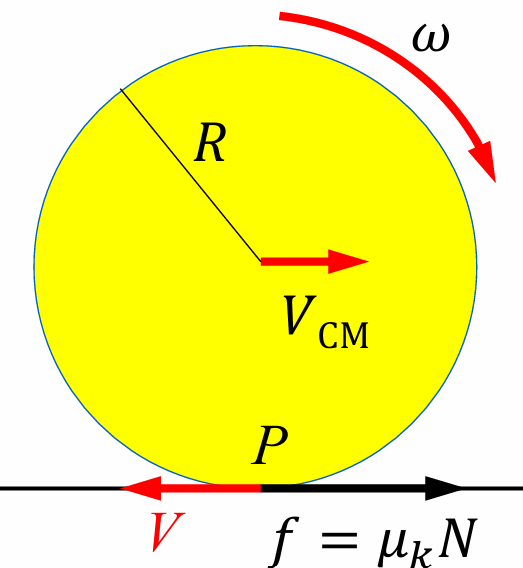
\includegraphics[width=0.3\linewidth]{images/rolling with slipping 2.png}
    \end{center}
    If CM at centre:
    \[
    \begin{aligned}
        M\dv{V_{\text{CM}}}{t} &= f \\
        I\dv{\omega}{t} &= -fR
    \end{aligned}
    \]
    Thus, $V_{\text{CM}}$ increases and $\omega$ decreases until $V_{\text{CM}} = R\omega$
    \item Example: Getting Up To Speed \\
    Assuming CM at centre, initially rolling with slipping: what's the final velocity? \\ \vspace{5pt}
    Pick z-axis to be parallel to ground
    \begin{center}
        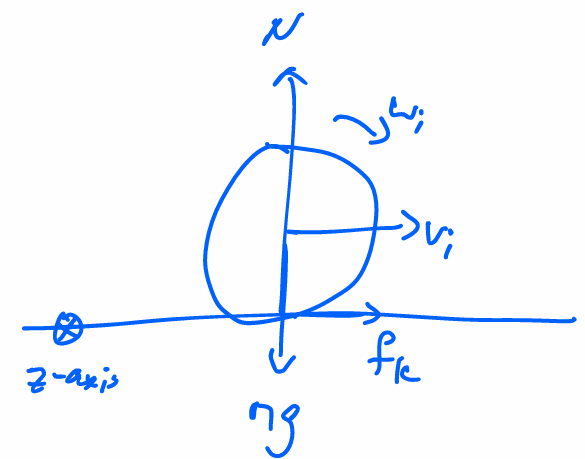
\includegraphics[width=0.5\linewidth]{images/getting up to speed.png}
    \end{center}
    Recap (rolling without slipping): $\tau_{\text{net}} = 0$ as $\tau_{\text{N}} + \tau_{\text{mg}} = 0$ and $\tau_{\text{fric}} = 0$
    By CoAM,
    \[
    \begin{aligned}
        L_i &= L_f \\
        RMv_i + I_{\text{CM}}\omega_i &= RMv_f + I_{\text{CM}}\omega_f \\
        &= \left( RM + \frac{I_{\text{CM}}}{R} \right) v_f \\
        \Rightarrow v_f &= \frac{RM + \frac{I_{\text{CM}}}{R}}{RMv_i + I_{\text{CM}}\omega_i}
    \end{aligned}
    \]
    Note: After a period of time, the ball will reach no-slipping condition hence $v_f = R\omega_f$ \\ \vspace{5pt}
    Alternatively, pick z-axis along the CM
    \begin{center}
        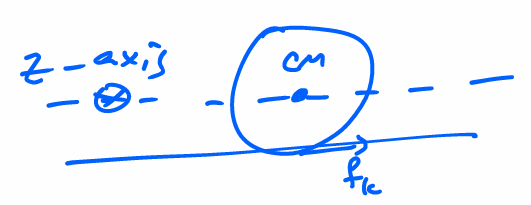
\includegraphics[width=0.6\linewidth]{images/getting up to speed 2.png}
    \end{center}
    \[
    \begin{aligned}
        L_i &= 0 + L_{\text{int, i}} = I_{\text{CM}}\omega_i \\
        L_f &= I_{\text{CM}}\omega_f \\
        \abs{\vb{r}_{\text{fric}} \cross \vb{f}_k} &= \abs{Rf_k}
    \end{aligned}
    \]
    According to sign convention,
    \[
    \begin{aligned}
        \tau_{\text{fric}} &= -Rf_k \\
        M\dv{v_{\text{CM}}}{t} &= f_k \\
        \Rightarrow v_f - v_i &= \int_{t_i}^{t_f} \frac{f_k}{M} \ dt \\
        \dv{v_{\text{CM}}}{t} &= \tau_{\text{net}} = Rf_k \\
        \Rightarrow L_f - L_i &= \int_{t_i}^{t_f} -Rf_k \ dt \\
        L_f - L_i &= -RM(v_f - v_i) \\        
    \end{aligned}
    \]
    Hence,
    \[
    \begin{aligned}
        I_{\text{CM}}(\omega_f - \omega_i) &= RM(v_i = v_f) \\
        I_{\text{CM}}\left( \frac{v_f}{R} - \omega_i \right) &= RM(v_i = v_f) \\
        \Rightarrow v_f &= \frac{RM + \frac{I_{\text{CM}}}{R}}{RMv_i + I_{\text{CM}}\omega_i}
    \end{aligned}
    \]
    \item Gyroscope, Falling
    \begin{center}
        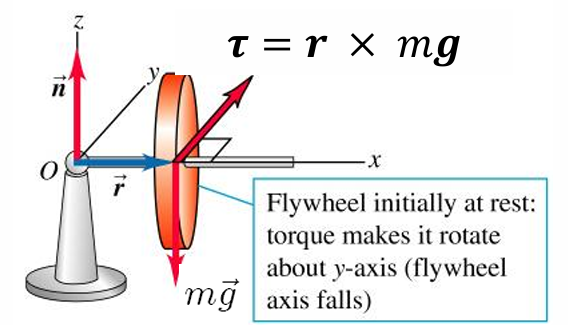
\includegraphics[width=0.5\linewidth]{images/gyroscope falling.png}
    \end{center}
    If the wheel is not spinning, it falls down due to gravity
    \begin{itemize}
        \item Torque due to $mg$, $\vb{\tau} = \vb{r} \cross m\vb{g}$
        \item $L_i = 0$, so $\vb{\dot{L}}(t)$ will be in the direction of $\vb{\tau}$, thus it rotates about $\vb{\tau}$
    \end{itemize}
    \item Gyroscope, Precessing
    \begin{center}
        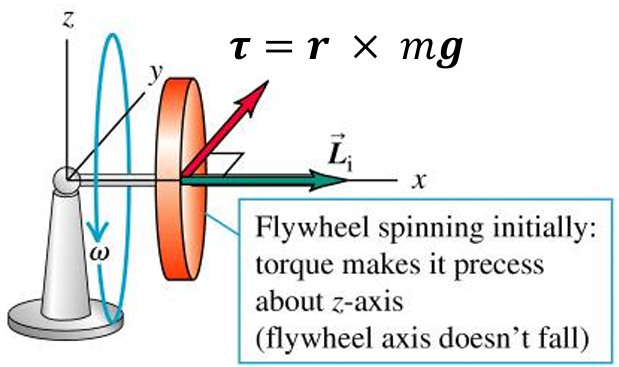
\includegraphics[width=0.5\linewidth]{images/gyroscope precessing.png}
    \end{center}
    \begin{center}
        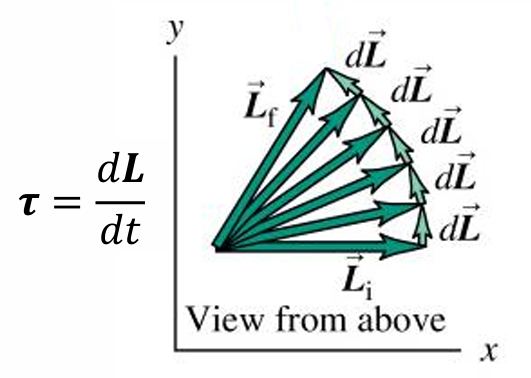
\includegraphics[width=0.4\linewidth]{images/gyroscope precessing graph.png}
    \end{center}
    When the wheel is spinning,
    \begin{itemize}
        \item Initial angular momentum $\vb{L}_i \neq 0$ is directed along x-axis
        \item The torque magnitude remains $\abs{\tau}=mgr$ and $\vb{\tau} \perp \vb{L_i}$
        \item Since $\vb{\tau} = \dv{\vb{L}}{t} = \vb{\Omega}_{\text{prec}} \cross \vb{L}$, $\vb{\Omega}_{\text{prec}}$ is in the +z-direction so the axle rotates around the z-axis
        \item Torque does not change the magnitude of $\vb{L}$, instead it causes $\vb{L}$ to change direction, i.e., $\vb{L}$ will precess about the z-axis
    \end{itemize}
    \item Gyroscope, Nutating
    \begin{center}
        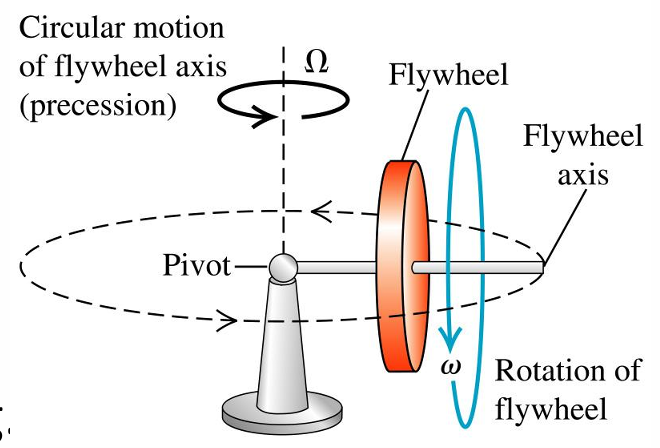
\includegraphics[width=0.5\linewidth]{images/gyroscope nutating.png}
    \end{center}
    Once it starts precessing,
    \begin{itemize}
        \item It yields wiggling movements called nutation
        \item If $\abs{\vb{\omega}} \gg \abs{\vb{\Omega}}$, then $\vb{L} \approx I\vb{\omega}$
    \end{itemize}
    \begin{center}
        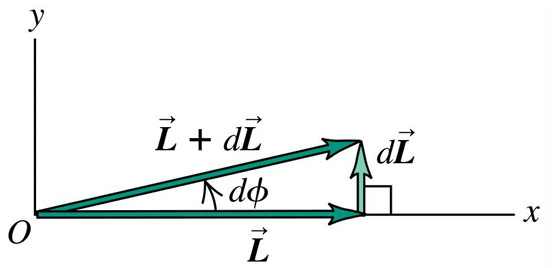
\includegraphics[width=0.5\linewidth]{images/gyroscope ignore nutation.png}
    \end{center}
    \begin{itemize}
        \item Choose axes so $\vb{\Omega} = \Omega\uvec{k}$ and $\vb{\omega}_{\text{spin}} = \omega_{\text{spin}}\uvec{e}$ for $\uvec{e}$ in x-y plane
        \item We can observe that $\frac{dL}{L} = d\phi \Rightarrow \frac{1}{L}\dv{L}{t} = \dv{\phi}{t} = \Omega$
        \item Also, $\vb{\tau} = \dv{\vb{L}}{t} \Rightarrow mgr = \dv{L}{t}$
        \item Hence, $\Omega$ is larger when $\omega_{\text{spin}}$ is smaller as long as $\abs{\vb{\omega}_{\text{spin}}} \gg \abs{\vb{\Omega}}$ still holds: $\Omega \approx \frac{mgr}{I\omega_{\text{spin}}}$
    \end{itemize}
\end{itemize}

% ====================================================
%                      Chapter 6
% ====================================================

\section{6. Lagrangian Mechanics}
\subsection{Euler-Lagrange Equations}
\begin{itemize}
    \item Denote $V$ as the potential and $r_j$ for the coordinates: $F_j = -\pdv{V}{r_j}$
    \item By Newton's second law, for each component: $m\ddot{r}_j = F_j^{\text{net}} = -\pdv{V}{r_j}$
    \item For particle in 1D, under (only) conservative forces, define Lagrangian $\mathcal{L} = T - V$, where $T = \frac{1}{2}m\dot{x}^2$ is KE
    \item Rewrite the second law $m\ddot{x} = -\pdv{V}{x}$:
    \[
    \begin{aligned}
        m\ddot{x} &= \dv{t}(m\dot{x}) = \dv{t}\left( \pdv{\dot{x}}\left( \frac{1}{2}m\dot{x}^2 - V \right) \right) = \dv{t}\left( \pdv{\mathcal{L}}{\dot{x}} \right) \\
        -\pdv{V}{x} &= \pdv{x}\left( \frac{1}{2}m\dot{x}^2 - V \right) = \pdv{\mathcal{L}}{x} \\
        \Rightarrow \dv{t}\left( \pdv{\mathcal{L}}{\dot{x}} \right) &= \pdv{\mathcal{L}}{x}
    \end{aligned}
    \]
    \item For particle in 3D, use the same technique to obtain $\dv{t}\left( \pdv{\mathcal{L}}{\dot{r}_j} \right) = \pdv{\mathcal{L}}{r_j}$
    \item This equation can be applied to any coordinate system
    \item Example: Simple Pendulum
    \begin{center}
        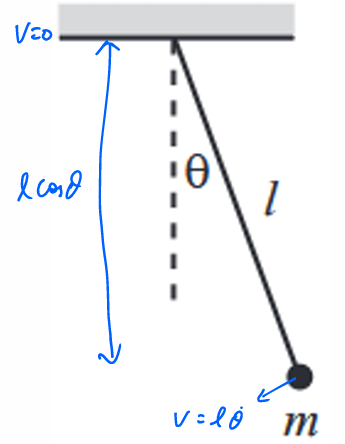
\includegraphics[width=0.3\linewidth]{images/simple pendulum.png}
    \end{center}
    \[
    \begin{aligned}
        \mathcal{L} &= T - V = \frac{1}{2}mv^2 - (-mgl\cos\theta) = \frac{1}{2}ml^2\dot{\theta}^2 + mgl\cos\theta \\
        \dv{t}\left( \pdv{\mathcal{L}}{\dot{\theta}} \right) &= \dv{t}\left( \frac{1}{2}ml^2 (2\dot{\theta}) \right) = ml^2\ddot{\theta} \\
        \pdv{L}{\theta} &= -mgl\sin\theta
    \end{aligned}
    \]
    Setting them equal:
    \[
    \begin{aligned}
        ml^2\ddot{\theta} &= -mgl\sin\theta \\
        \ddot{\theta} &= -\frac{g}{l}\sin\theta
    \end{aligned}
    \]
    \item Principle of Stationary Action: Of all possible paths connecting the same initial and final configurations at fixed times, the actual path is one for which the action does not change to first order under a small variation of the path (i.e. $\delta S = 0$)
    \item Action, $S = \int_{t_i}^{t_f} \mathcal{L} \ dt = \int_{t_i}^{t_f} (T - V) \ dt$
    \item We assume that if the particle(s) are described by coordinates ${q_j(t)}$, $\mathcal{L}$ is only a function of these $q_j$, their first time derivatives, and time: $\mathcal{L} = \mathcal{L}(q_j, \dot{q}_j, t)$
    \item If some trajectory(s) give a stationary point of action, then it satisfies the \bf{Euler-Lagrange Equation}: $\dv{t}\left(\pdv{\mathcal{L}}{\dot{q}_j}\right) = \pdv{\mathcal{L}}{q_j}$
    \item If we set $\mathcal{L}(q_j, \dot{q}_j, t) = T - V$, then particles will follow trajectories s.t. $\int_{t_i}^{t_f} \mathcal{L}(q_j, \dot{q}_j, t) \ dt$ is a stationary point, which also implies the Euler-Lagrange equation hold
    \item When the qn ask for equations of motion, it suffice to show the differential equations involving the respective coordinates
\end{itemize}

\subsection{Noether's Theorem}
\begin{itemize}
    \item Example: Uniform Gravity
    A particle is subject to uniform gravity $\vb{F}_g = -mg\uvec{k}$. Using the lagrangian method, find the equations of motion. \\
    \[
    \begin{aligned}
        T &= \frac{1}{2}m(\dot{r}_1^2 + \dot{r}_2^2 + \dot{r}_3^2) \\
        V &= mgr_3 \\
        T - V &= \frac{1}{2}m(\dot{r}_1^2 + \dot{r}_2^2 + \dot{r}_3^2) - mgr_3 \\
        \dv{t}\left( \pdv{\mathcal{L}}{\dot{r}_3} \right) &= \dv{t}(m\dot{r}_3) = m\ddot{r}_3 \\
        \pdv{\mathcal{L}}{r_3} &= -mg \\
        \Rightarrow \ddot{r}_3 &= -g, \ddot{r}_1 = 0, \ddot{r}_2 = 0
    \end{aligned}
    \]
    This also mean $\pdv{\mathcal{L}}{\dot{r}_1}$ and $\pdv{\mathcal{L}}{\dot{r}_2}$ are constant
    \item Example: Conical Pendulum
    \begin{center}
        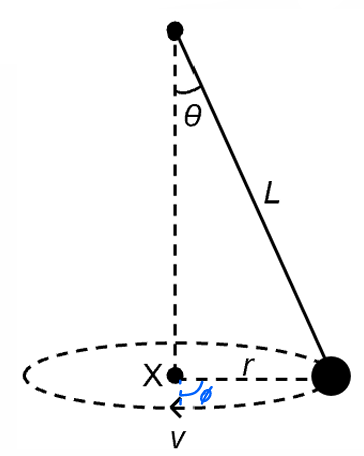
\includegraphics[width=0.3\linewidth]{images/conical pendulum.png}
    \end{center}
    \[
    \begin{aligned}
        T &= \frac{1}{2}m\left(L^2\dot{\theta}^2 + L^2\sin^2\theta \ \dot{\phi}^2\right) \text{ (contribution from $v_\theta$ and $v_\phi$)} \\
        V &= -mgL\cos\theta \\
        \mathcal{L} &= \frac{1}{2}m\left(L^2\dot{\theta}^2 + L^2\sin^2\theta \ \dot{\phi}^2\right) + mgL\cos\theta \\
        \dv{t}\left(\pdv{\mathcal{L}}{\dot{\theta}}\right) &= \dv{t}(mL^2\dot{\theta}) = mL^2\dot{\theta} \\
        \pdv{\mathcal{L}}{\theta} &= mL^2\sin\theta\cos\theta \ \dot{\phi}^2 - mgL\sin\theta \\
        \dv{t}\left(\pdv{\mathcal{L}}{\dot{\theta}}\right) &= \dv{t}(mL^2\sin^2\theta \ \dot{\phi}) \\
        \pdv{\mathcal{L}}{\phi} &= 0
    \end{aligned}
    \]
    This means that $mL^2\sin^2\theta \ \dot{\phi}$ is constant
    \item Noether's Theorem: every "continous symmetry" in a physical system corresponds to a conserved quantity, and vice versa \\
    \begin{center}
        $\mathcal{L}$ has no "explicit" dependence on coordinate $q_j$ \\
        $\Leftrightarrow \dv{t}\left(\pdv{\mathcal{L}}{\dot{q}_j}\right) = \pdv{\mathcal{L}}{q_j} = 0$ \\
        $\Leftrightarrow \pdv{\mathcal{L}}{\dot{q}_j}$ is a conserved quantity
    \end{center}
    \begin{itemize}
        \item Independent of Cartesian coord $r_j \Leftrightarrow$ translation symmetry along that direction $\Leftrightarrow$ conservation of linear momentum
        \item Independent of Angular coord $\theta \Leftrightarrow$ rotation symmetry w.r.t. an axis $\Leftrightarrow$ conservation of angular momentum w.r.t. that axis
    \end{itemize}
    \item Such a coordinate $q_j$ is called a cyclic coordinate
    \item Maxwell's equations are frame independent $\Leftrightarrow$ light speed is constant (No-ether theorem)
    \item When $\mathcal{L}$ has no "explicit" time dependence, $\pdv{\mathcal{L}}{t} = 0 \Leftrightarrow \underset{j}{\sum}\left(\pdv{\mathcal{L}}{\dot{q}_j} \dot{q}_j\right) - \mathcal{L} = \text{const}$
    \item We can show this by proving $\dv{t}\left(\sum_j\left(\pdv{\mathcal{L}}{\dot{q}_j} \dot{q}_j\right) - \mathcal{L}\right) = -\pdv{\mathcal{L}}{t}$ (note: LHS is total derivative):
    \[
    \begin{aligned}
        \text{LHS} &= \sum_j\left( \left(\dv{t}\pdv{\mathcal{L}}{\dot{q}_j}\right) + \pdv{\mathcal{L}}{\dot{q}_j}\ddot{q}_j \right) - \dv{\mathcal{L}}{t} \\
        &= \sum_j\left( \left(\dv{t}\pdv{\mathcal{L}}{\dot{q}_j}\right) + \pdv{\mathcal{L}}{\dot{q}_j}\ddot{q}_j \right) - \left( \sum_j \left( \pdv{\mathcal{L}}{q_j}\dot{q}_j + \pdv{\mathcal{L}}{\dot{q}_j}\ddot{q}_j\right) + \pdv{\mathcal{L}}{t} \right) \\
        &= \sum_j \left( \left( \dv{t}\pdv{\mathcal{L}}{\dot{q}_j} - \pdv{\mathcal{L}}{q_j} \right)\dot{q}_j \right) -\pdv{\mathcal{L}}{t} \\
        &= -\pdv{\mathcal{L}}{t} \text{ (by E-L eqns)}
    \end{aligned}
    \]
    \item We can check that e.g. for $\mathcal{L} = T - V$ with $V$ depending only on particle position(s), we have in Cartesian coords $\mathcal{L} = \frac{1}{2}m\sum_j\dot{q}_j^2 - V(q_j)$, and so:
    \[
    \begin{aligned}
        \sum_j\left(\pdv{\mathcal{L}}{\dot{q}_j}\dot{q}_j\right) - \mathcal{L} &= \sum_j \left((m\dot{q}_j)\dot{q}_j\right) - \mathcal{L} \\
        &= 2T - \mathcal{L} \\
        &= T + V
    \end{aligned}
    \]
    \item If $\sum_j\left(\pdv{\mathcal{L}}{\dot{q}_j}\dot{q}_j\right) - \mathcal{L}$ is a constant, we get a constant $T + V$, meaning energy is conserved (mostly true, unless $\mathcal{L} \neq T - V$).  
\end{itemize}

% ====================================================
%                      Chapter 7
% ====================================================

\section{7. Central Forces}
\begin{itemize}
    \item A central force is a force which (for a fixed length of origin), always point towards/away the origin and only depends on distance from origin
    \item This means $\vb{F} = f(r)\uvec{r}$, where $f(r)$ is a function of (only) distance $r$ from origin
    \item Since torque exerted by central force is $\vb{\tau} = \vb{r}\cross\vb{F} = \vb{r}\cross f(r)\uvec{r} = 0$, angular momentum is always conserved
    \item Kepler's 2nd Law:
    \begin{center}
        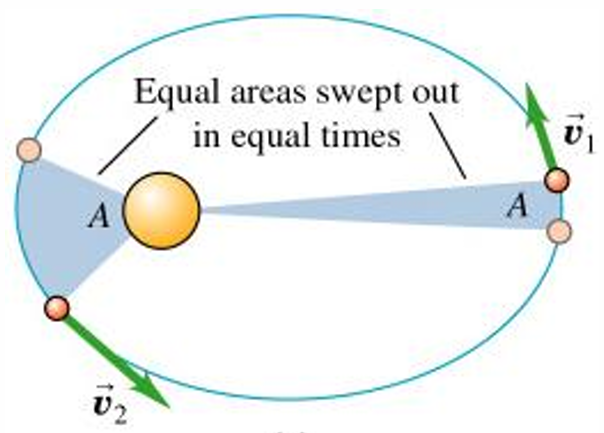
\includegraphics[width=0.5\linewidth]{images/kepler second law.png}
    \end{center}
    \item It turns out to be CoAM in disguise
    \begin{center}
        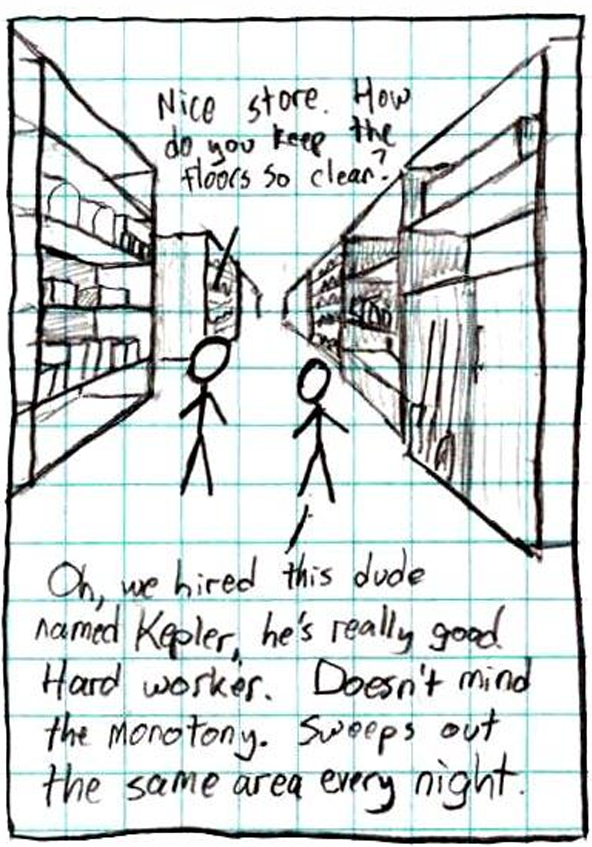
\includegraphics[width=0.3\linewidth]{images/kepler meme.png}
    \end{center}
    \item We found that the point mass stays in the plane, so we basically have a scalar $L$ since the vector $L$ is always perpendicular to the plane
    \begin{center}
        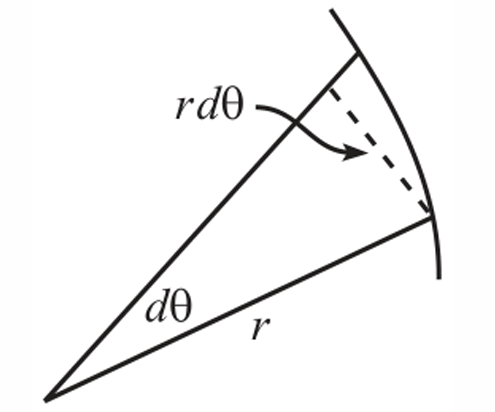
\includegraphics[width=0.4\linewidth]{images/kepler second law triangle.png}
    \end{center}
    \item Recall that $L = mr^2\dot{\theta}$. By calculating the area of triangle, we get
    \[
    \begin{aligned}
        dA &= \frac{1}{2}r(rd\theta) \\
        \Rightarrow \dv{A}{t} &= \frac{1}{2}r^2\dv{\theta}{t} = \frac{L}{2m}
    \end{aligned}
    \]
    \item So $\dv{A}{t}$ is constant $\Leftrightarrow$ $L$ is constant
    \item We know that conservative force $\coloneqq$ work done is path-independent. Informal "brute-force" proof:
    \begin{center}
        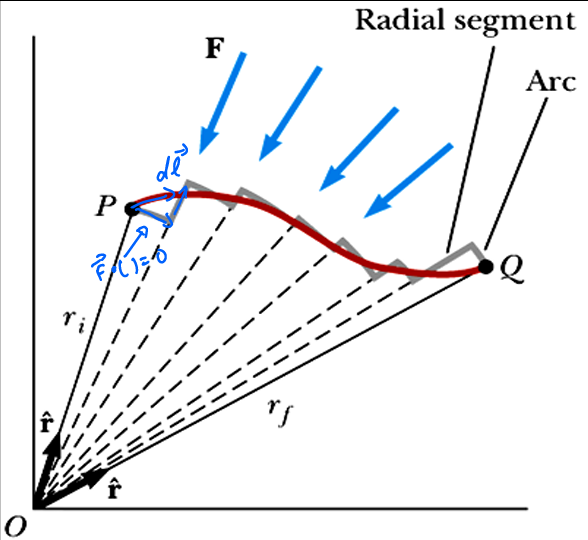
\includegraphics[width=0.4\linewidth]{images/central forces conservative graph.png}
        \[
            W = \int_P^Q \vb{F}\cdot d\vb{l} = \int_{r_i}^{r_f} F(r) \ dr
        \]
    \end{center}
    only depends on $r_i$ and $r_f \Rightarrow$ only depends on $P$ and $Q$
    \item Alternatively, we can look at central force potentials: \\
    If a potential has form $U(r)$ where $r = \sqrt{x^2 + y^2 + z^2}$, then
    \[
    \begin{aligned}
        -\pdv{U}{x} = -\pdv{r}{x}U'(r) = -\frac{1}{2}\frac{2x}{\sqrt{x^2 + y^2 + z^2}}U'(r) = -\frac{x}{\sqrt{x^2 + y^2 + z^2}}
    \end{aligned}
    \]
    So
    \[
    \begin{aligned}
        \vb{F} = -\frac{U'(r)}{\sqrt{x^2 + y^2 + z^2}}(x\uvec{i} + y\uvec{j} + z\uvec{k}) = -\frac{U'(r)}{r}\vb{r} = -U'(r)\uvec{r}
    \end{aligned}
    \]
    Now, flip it around: given a central force in the form $\vb{F} = f(r)\uvec{r}$, any $U(r)$ such that $U'(r) = -f(r)$ is a valid potential. \\
    Hence, central forces are conservative. \\
    note: This only require $U(r)$ to be an indefinite integral of $f(r)$, i.e. $U(r) = \int f(r) \ dr$
    \item Now suppose $U(r)$ is the potential for central force; use polar coords $(r, \theta)$ in the plane of motion:
    \[
    \begin{aligned}
        \mathcal{L} &= \frac{1}{2}m(\dot{r}^2 + r^2\dot{\theta}^2) - U(r)
    \end{aligned}
    \]
    This doesn't depend on $\theta$, i.e. $\theta$ is a cyclic coordinate $\Rightarrow \pdv{\mathcal{L}}{\dot{\theta}}$ is a conserved quantity
    \[
    \begin{aligned}
        \dv{t}\left(\pdv{\mathcal{L}}{\dot{r}}\right) &= \dv{t}(m\dot{r}) = m\ddot{r} \\
        \pdv{\mathcal{L}}{r} &= mr\dot{\theta}^2 - U'(r) \\
        \Rightarrow m\ddot{r} = mr\dot{\theta}^2 - U'(r) &\text{ and } mr^2\dot{\theta} = \text{const}
    \end{aligned}
    \]
    \item We can see that the conserved quantity $mr^2\dot{\theta}$ is just the angular momentum $L$
    \item Sub $\dot{\theta} = \frac{L}{mr^2}$ and let $m\ddot{r} = -U'_{\text{eff}}(r)$, we get the equations:
    \[
    \begin{aligned}
        m\ddot{r} &= \frac{L^2}{mr^3} - U'(r) = -U'_{\text{eff}}(r), \\
        U_{\text{eff}}(r) &\coloneqq \frac{L^2}{2mr^2} + U(r),
    \end{aligned}
    \]
    where $\frac{L^2}{2mr^2}$ is the "angular momentum barrier"
    \begin{center}
        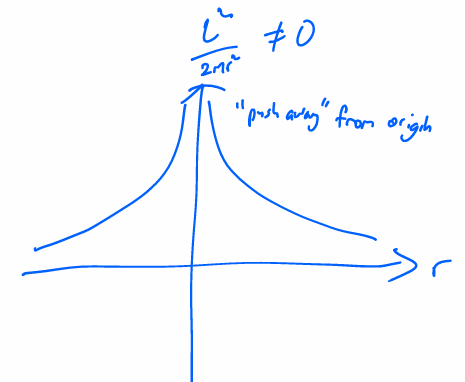
\includegraphics[width=0.5\linewidth]{images/angular momentum barrier.png}
    \end{center}
    \item i.e. radial coord $r$ behaves like 1D motion under the effective potential $U_{\text{eff}}(r)$
    \item Total energy $E$ is also conserved:
    \[
    \begin{aligned}
        0 &= m\ddot{r} - \frac{L^2}{mr^3} + U'(r) \\
        &= m\ddot{r}\dot{r} - \frac{L^2}{mr^3}\dot{r} + U'(r)\dot{r} \\
        &= \dv{t}\left(\frac{1}{2}m\dot{r}^2 + \frac{L^2}{2mr^2} + U(r)\right) \\
        \Rightarrow &\frac{1}{2}m\dot{r}^2 + \frac{L^2}{2mr^2} + U(r) = \frac{1}{2}m\dot{r}^2 + U_{\text{eff}}(r) = E = \text{const}
    \end{aligned}
    \]
    \item We now have a differential equation for $\frac{1}{2}m\dot{r}^2 + U_{\text{eff}}(r) = E$ (or $m\ddot{r} = -U'_{\text{eff}}(r)$) for $r$
    \item If we have a solution for $r(t)$, we can get $\theta(t)$ by solving the other equation:
    \[
    \begin{aligned}
        mr^2\dot{\theta} &= L \\
        \Rightarrow \dot{\theta} &= \frac{L}{mr^2} \\
        \Rightarrow \theta(t) &= \int_0^t \frac{L}{m(r(t))^2} \ dt'
    \end{aligned}
    \]
    \item If we want the "shape" of the particle in space, 
    \[
    \begin{aligned}
        \frac{1}{2}m\dot{r}^2 + U_{\text{eff}}(r) = E &\Rightarrow \dot{r}^2 = \frac{2(E - U_{\text{eff}}(r))}{m} \\
        mr^2\dot{\theta} = L &\Rightarrow r^4\dot{\theta}^2 = \frac{L^2}{m^2} \\
        \Rightarrow \frac{1}{r^4}\left(\dv{r}{\theta}\right)^2 &= \frac{2m(E - U_{\text{eff}}(r))}{L^2}
    \end{aligned}
    \]
    For edge case $L = 0$, we can treat it as a 1D motion and handle it separately.
    \item Example: Inverse-Square Force (Attractive)
    \begin{center}
        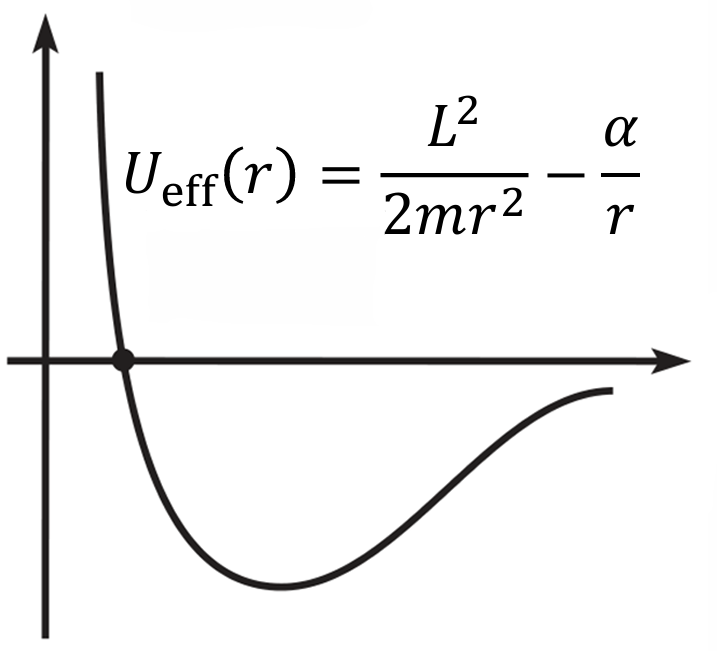
\includegraphics[width=0.4\linewidth]{images/inverse square law attractive.png}
    \end{center}
    When $E \geq 0$, we get \textbf{unbound} orbits/trajectories
    \begin{center}
        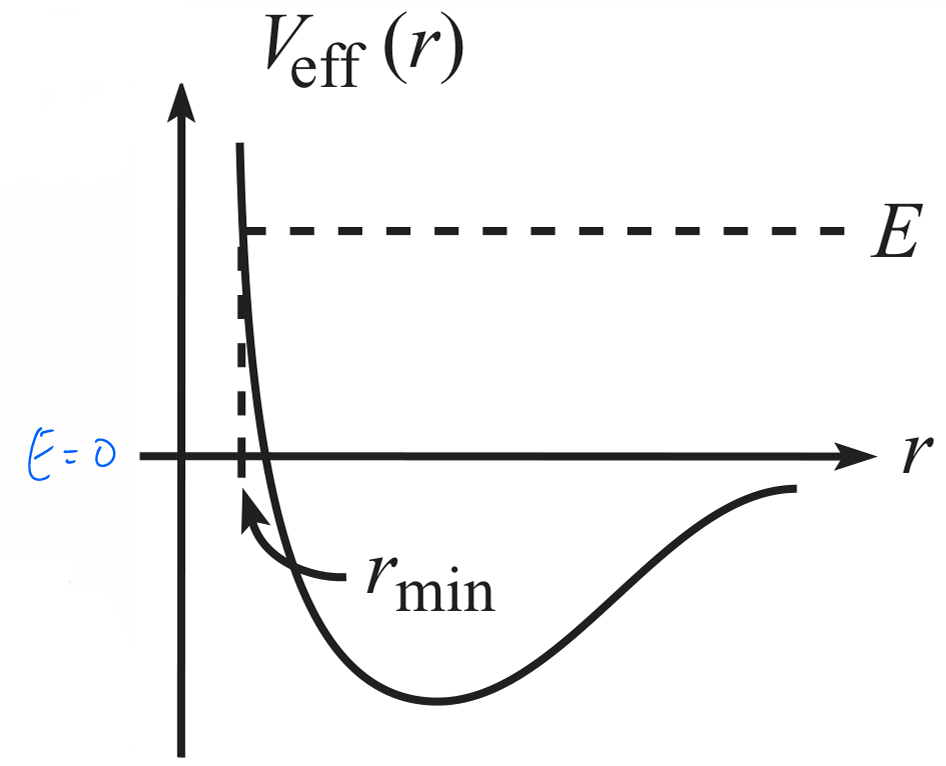
\includegraphics[width=0.48\linewidth]{images/inverse square law unbound.png}
    \end{center}
    \begin{itemize}
        \item There's a minimum $r$ value
        \item For $E = 0$, the particle escapes to infinity
        \item For inverse-square $-\frac{\alpha}{r^2}\uvec{r}$, this trajectory is "symmetric" (hyperbola for $E > 0$ and parabola for $E = 0$)
    \end{itemize}
    When $E < 0$, we get \textbf{bound} orbits/trajectories
    \begin{center}
        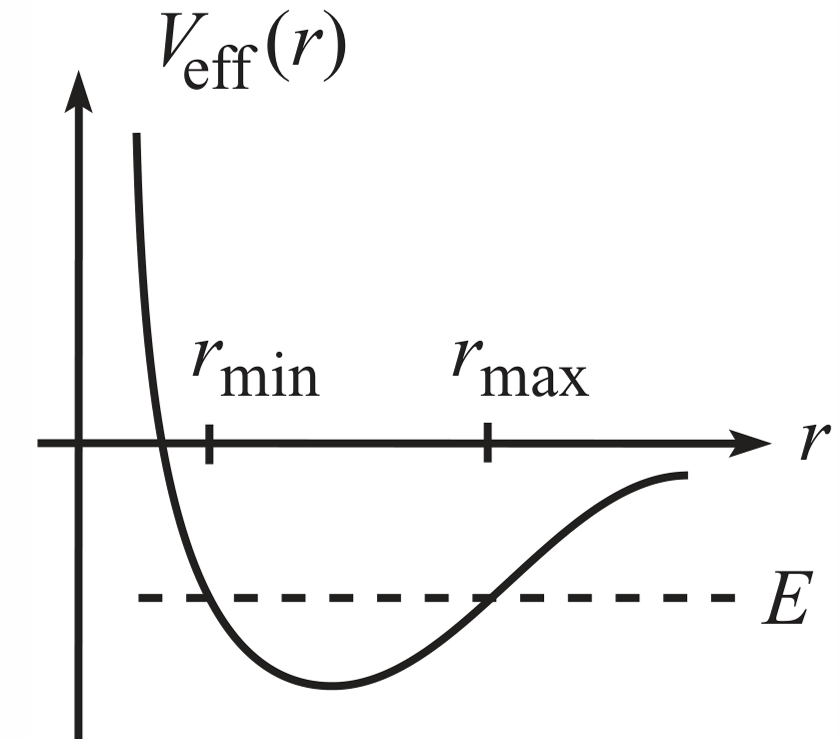
\includegraphics[width=0.45\linewidth]{images/inverse square law bound.png}
    \end{center}
    \begin{itemize}
        \item Particle oscillates between min/max $r$ values
        \item The orbit is ellipse shaped
    \end{itemize}
    \item When $E = \text{min value of }U_{\text{eff}}$ (which is $-\frac{m\alpha^2}{2L^2}$),
    \begin{center}
        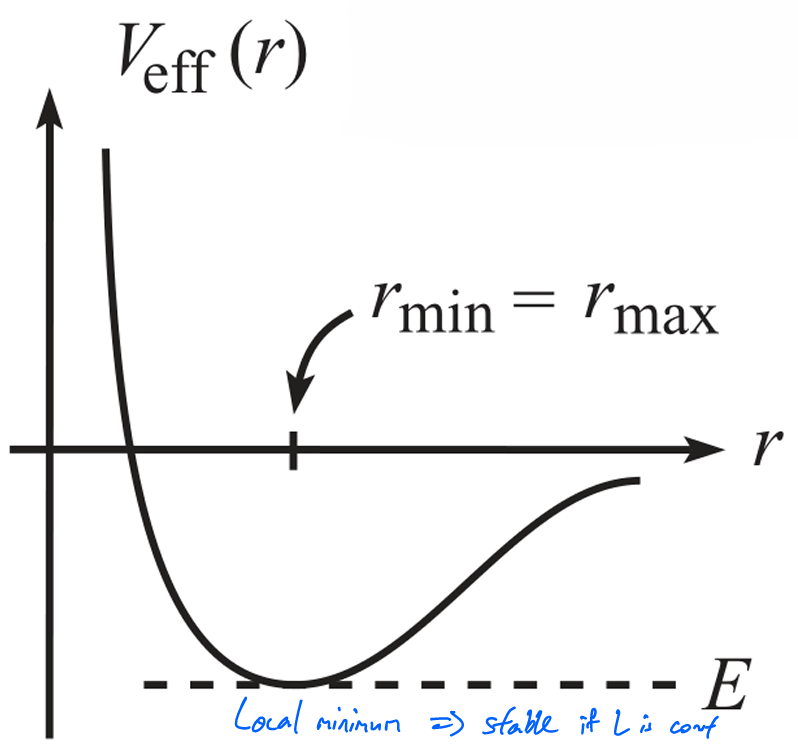
\includegraphics[width=0.45\linewidth]{images/inverse square law min.png}
    \end{center}
    \begin{itemize}
        \item $r$ remains constant at equilibrium
        \item Particle in circular orbit $\Leftrightarrow \abs{\text{centripetal force}} = \abs{f(r)} = \abs{U'(r)}$
        \item If slightly perturbed, the orbit become ellipse shaped
    \end{itemize}
    \item Note that this is not generalizable to all cases of $U(r)$, e.g.:
    \begin{itemize}
        \item Could be less than/more than 1 equilibrium point
        \item "Threshold" for escaping may be $E = \underset{r \rightarrow \infty}{\lim}U_{\text{eff}}(r)$ (which is same as $\underset{r \rightarrow \infty}{\lim}U(r)$ because $r \rightarrow \infty$ means $\frac{L^2}{2mr^2} \rightarrow \infty$ as well)
        \item Particle might be "locally" trapped as well, e.g. having a peak between the 0 and infinity and not enough energy to overcome this peak to go to infinity
        \item If $U(r)$ diverges "fast enough" as $r \rightarrow \infty$, may outweight the angular momentum barrier
        \item etc
    \end{itemize}
    \item Two-Body Problem: trick is to consider one particle's frame of reference
    \begin{itemize}
        \item Consider two object with mass $M$ and $m$
        \item In $M\text{'s}$ frame, $m\text{'s}$ acceleration is $\frac{\vb{F}}{m} - \frac{-\vb{F}}{M} = \left(\frac{m + M}{mM}\right)\vb{F}$
        \item Hence, we can rewrite $\ddot{r}^{\text{rel}} = \frac{\vb{F}}{\mu}$, where $\mu = \frac{mM}{m + M}$ and $\mu$ is called reduced mass (also always $< m$)
    \end{itemize}
    \item Note that if $\vb{F}$ only depends on distance $\abs{\vb{r}^{\text{rel}}}$ between particles, it becomes a central-force problem since $\vb{F}$ is collinear to $\vb{r}^{\text{rel}}$ by assumption
    \item CM + relative position: given $\vb{r}_{\text{CM}}$ and $\vb{r}^{\text{rel}}$, recall:\\ 
    \begin{center}
        $\vb{r}_{\text{CM}} = \frac{M\vb{R} + m\vb{r}}{M + m}, \qquad \vb{r}^{\text{rel}} = \vb{r} - \vb{R}$
    \end{center}
    We can solve it algebraically to get $r$ and $R$
\end{itemize}

% ====================================================
%                      Chapter 8
% ====================================================

\section{8. Gravity}
\subsection{Newtonian Formulation}
\begin{itemize}
    \item Newton's Law of Universal Gravitation: $\abs{\vb{F}_g} = \frac{Gm_1m_2}{r^2}$, where $G = (6.67 \pm 0.01)\cross 10^{-11}\ \text{Nm}^2\ \text{kg}^{-2}$
    \item Example: Thin Uniform Ring
    \begin{center}
        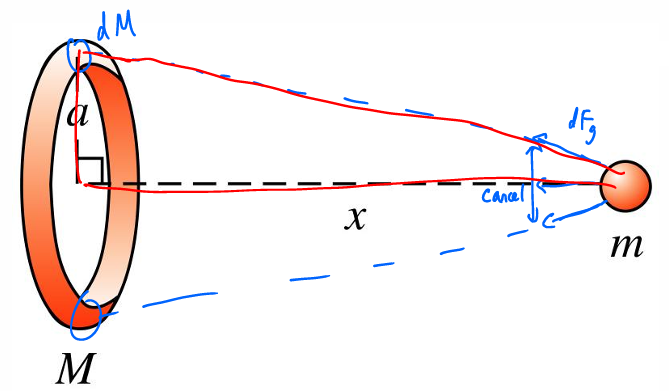
\includegraphics[width=0.6\linewidth]{images/thin uniform ring.png}
    \end{center}
    \begin{itemize}
        \item We can first see that the vertical component of $d\vb{F}_g$ cancels each other, leaving only the horizontal component to consider
        \item Next, the small triangle describing the infinitesimal gravitational force is similar to the larger triangle, so the magnitude is
    \end{itemize}
    \begin{center}
            $\abs{d\vb{F}_g}\frac{x}{\sqrt{x^2 + a^2}} = \frac{Gmx \ dM}{(x^2 + a^2)^{3/2}}$ \\
            $\abs{\vb{F}_g^{\text{horizontal}}} = \int_{\text{ring}} \frac{Gmx \ dm}{(x^2 + a^2)^{3/2}} = \frac{GMmx}{(x^2 + a^2)^{3/2}}$
    \end{center}
    \item Example: Thin Uniform Sphere
    \begin{center}
        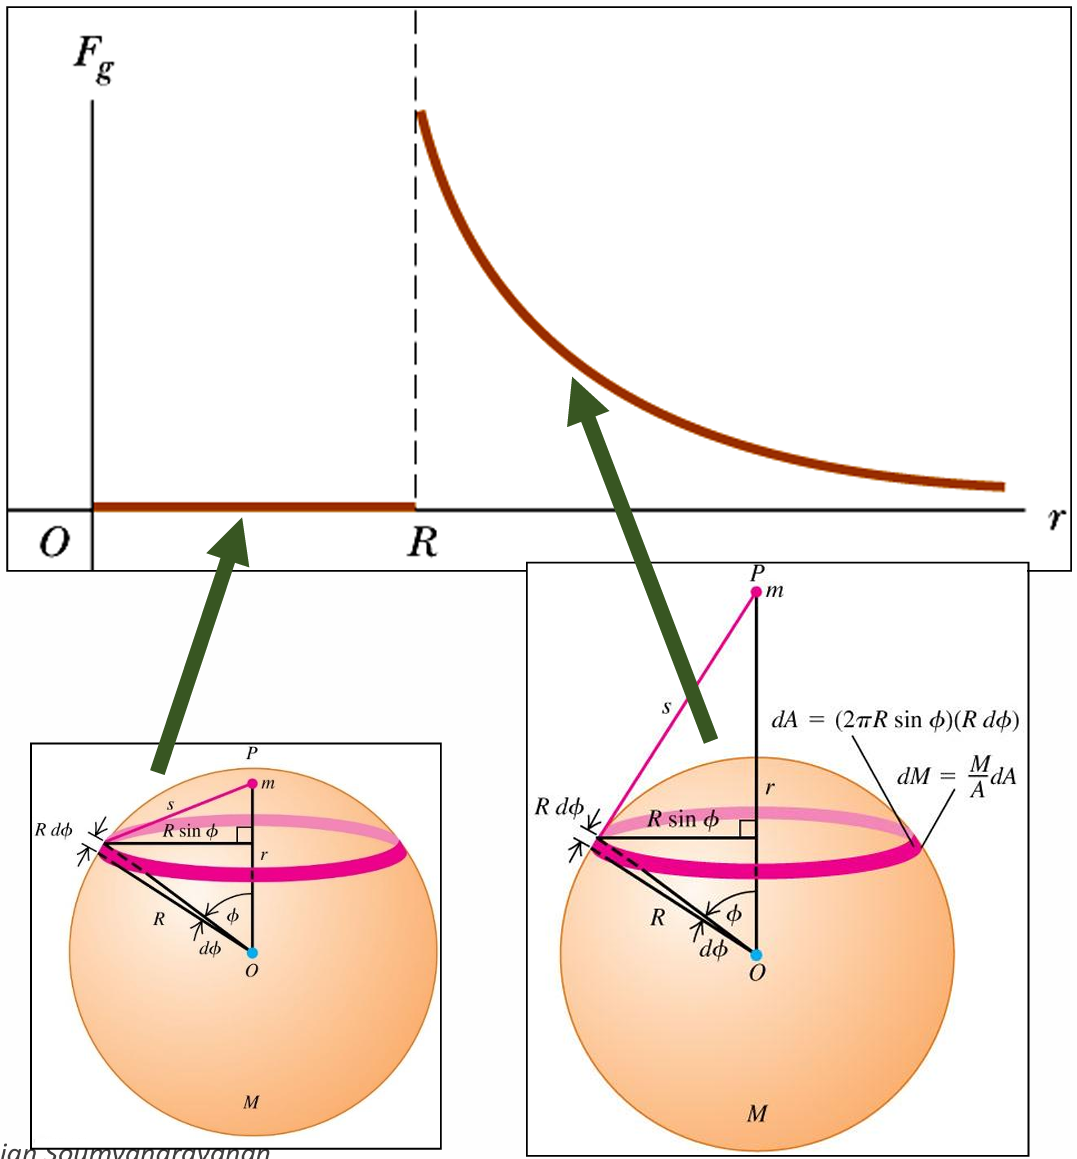
\includegraphics[width=0.9\linewidth]{images/thin uniform sphere.png}
    \end{center}
    \begin{itemize}
        \item Outside the sphere: same as a point mass at centre 
        \item Inside the sphere: zero
    \end{itemize}
    \begin{center}
        \[
        \vb{F}_g = 
        \begin{cases}
            -\frac{GMm}{r^2}\uvec{r} &, r > R \\
            \hspace{20pt} 0 &, r < R
        \end{cases}
        \]
    \end{center}
    \begin{itemize}
        \item This is sometimes called the shell theorem
        \item Proof delegated to the slides (too complicated to write here)
    \end{itemize}
    \item Example: Solid Uniform Ball
    \begin{center}
        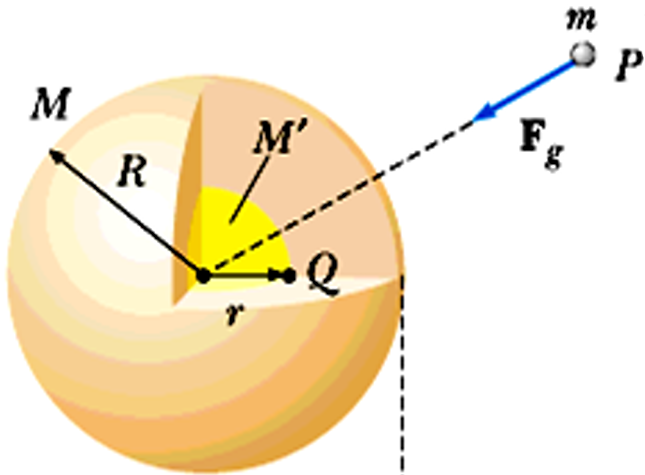
\includegraphics[width=0.5\linewidth]{images/solid uniform ball.png}
    \end{center}
    \begin{itemize}
        \item Divide the ball into concentric shells and use the previous results
        \item Outside the ball (e.g. point $P$), $\vb{F}_g = -\frac{GMm}{r^2}\uvec{r}$
        \item Inside the ball (e.g. point $Q$), mass $M' = M\left(\frac{r}{R}\right)^3$, thus $\vb{F}_g = -\frac{GM'm}{r^2}\uvec{r} = -\frac{GMmr}{R^3}\uvec{r}$
        \item The resulting graph:
    \end{itemize}
    \begin{center}
        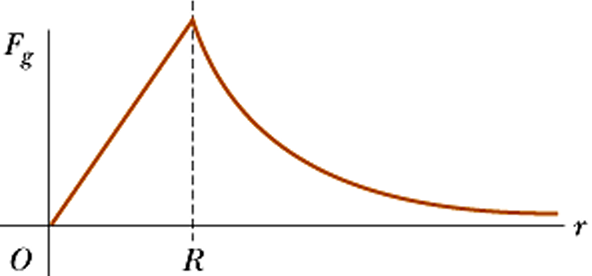
\includegraphics[width=0.6\linewidth]{images/solid uniform ball graph.png}
    \end{center}
    \item Gravitational Potential Energy: $U_g(r) = -\frac{GMm}{r}$
    \item The usual GPE convention is $U_g(r) \rightarrow 0$ as $r \rightarrow \infty$. In lab scenarios, objects are moving in very small range of $r$, so $\abs{\vb{F}_g} \approx \text{constant} = mg \Rightarrow$ potential is linear, denoted by mgh
    \item Consider the thin uniform ring example again, 
    \begin{center}
        $dV = -\frac{G(dM)m}{\sqrt{x^2+a^2}} \Rightarrow U = \int_{\text{ring}}-\frac{G(dM)m}{\sqrt{x^2+a^2}} = -\frac{GMm}{\sqrt{x^2+a^2}}$
    \end{center}
    Differentiating $U$ gives 
    \[
    \begin{aligned}
        F_x = -\pdv{U}{x} = GMm\left(-\frac{1}{2}\frac{2x}{(x^2+a^2)^{3/2}}\right) = -\frac{GMmx}{(x^2+a^2)^{3/2}}
    \end{aligned}
    \]
    This is consistent with the previous example. Technically, this computation is only valid on x-axis, but since the ring is a rigid body, we can leave out their "self energies" from GPE conputations
    \item When computing the GPE of a collection of point masses, we only count each pair once, e.g. if we have 4 point masses:
    \[
    \begin{aligned}
        U = U_{12} + U_{13} + U_{14} + U_{23} + U_{24} + U_{34}
    \end{aligned}
    \]
    \item Since rigid bodies means that the distances between each points in the bodies are fixed, the "self-energies" are constant and doesnt affect the "dynamics" (or EOM)    
\end{itemize}

\subsection{Astronomical Bodies, Orbits}
\begin{itemize}
    \item Escape speed is the minimum speed needed to escape from surface of mass $M$ and radius $R$: $v_i \geq v_{\text{esc}} = \sqrt{\frac{2GM}{R}}$
    \item This speed is independent of mass $m$ of escaping object and direction of $v_i$
    \item Fun fact: gas molecules have nonzero speeds from thermal motion $\Rightarrow$ increases w.r.t temp, decreases w.r.t. particle mass
    \item If "average" speed of some molecule (at planet's temp) exceeds escape speed, little is found on the planet. E.g. Mercury, Moon are "airless", Earth have very little hydrogen
    \item Consider black holes. If we have a loose handwavy idea that nothing can exceed speed of light $c$, then if a massive body has $v_{\text{esc}} > c$, nothing escapes it.
    \begin{center}
        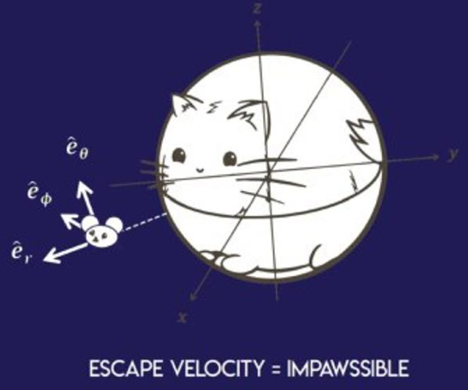
\includegraphics[width=0.4\linewidth]{images/black hole meme.png}
    \end{center}
    \item The relevant parameter to meet this condition is the $M/R$ ratio:
    \[
    \begin{aligned}
        c = \sqrt{\frac{2GM}{R}} \quad\Rightarrow\quad \frac{M}{R} = \frac{c^2}{2G}
    \end{aligned}
    \]
    note: its not about density as density is $\propto \frac{M}{R^3}$
    \item This is the case of right ans, wrong method! Just like how $\frac{1\cancel{6}}{\cancel{6}4} = \frac{1}{4}$
    \item Schwarzschild Radius: For a given $M$, can solve for critical $R$ at which it would be a black hole
    \begin{center}
        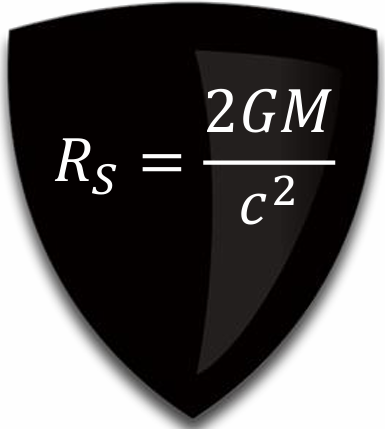
\includegraphics[width=0.25\linewidth]{images/schwarzschild radius.png}
    \end{center}
    \item Fun fact: Schwarzschild radius is called "black shield" if translated literally
    \item Example: Binary Stars (Circular Orbits) \\
    We want to show that each star has period $T^2 = \frac{4\pi^2d^3}{G(M + m)}$
    \begin{center}
        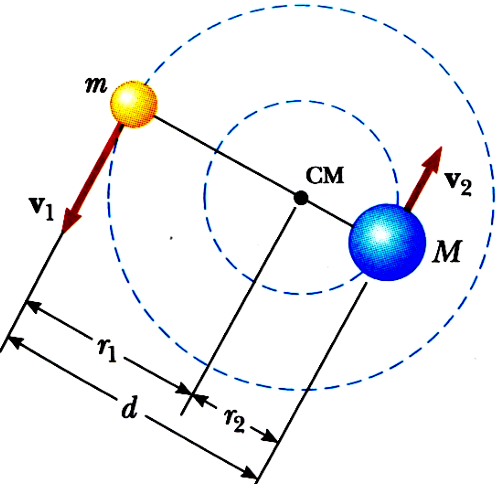
\includegraphics[width=0.4\linewidth]{images/binary stars circular orbit.png}
    \end{center}
    In inertial frame:
    
    For m, 
    \begin{center}
        $mr_1\omega_1^2 = \frac{GMm}{d^2} \quad \Rightarrow \quad \omega_1^2 = \frac{GM}{r_1d^2}$
    \end{center}
    
    For M, 
    \[
    \begin{aligned}
        Mr_2\omega_2^2 = \frac{GMm}{d^2} \quad \Rightarrow \quad \omega_2^2 = \frac{Gm}{r_2d^2} \\
        w_1 = w_2 \Rightarrow \frac{M}{r_1} = \frac{m}{r_2} \Rightarrow Mr_2 = mr_1
    \end{aligned}
    \]
    Since $r_1 + r_2 = d$, we have
    \[
    \begin{aligned}
        r_1 &= \frac{Md}{M + m} \\
        \Rightarrow \omega_1^2 &= \frac{GM}{r_1d^2} = \frac{G(M + m)}{d^3} \\
        \left(\frac{2\pi}{T}\right)^2 &= \frac{G(M + m)}{d^3} \Rightarrow T^2 = \frac{4\pi^2d^3}{G(M + m)}
    \end{aligned}
    \]
    \item Kepler's Laws
    \begin{enumerate}
        \item All planets move in \bf{elliptical orbits} with the Sun at one focus
        \item The radial vector drawn from the Sun to a planet sweeps out \bf{equal areas} in equal time intervals
        \item The \bf{square of the orbital period} is proportional to the \bf{cube of the semi-major axis} of the elliptical orbit
    \end{enumerate}
    \begin{center}
        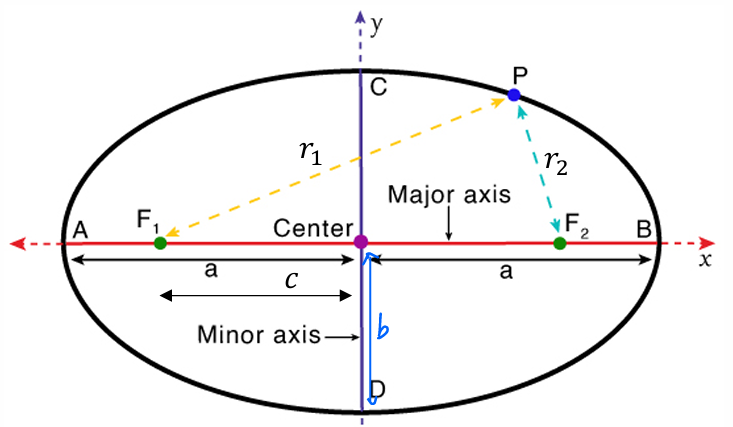
\includegraphics[width=0.7\linewidth]{images/ellipse.png}
    \end{center}
    \item Some properties for ellipse:
    \begin{itemize}
        \item If $a > b$, we call them semi-major axis $a$ and semi-minor axis $b$
        \item For 2 foci of equal distances from the center $F_1 \And F_2$, the sum of distances from the foci to any point on ellipse is constant: $r_1 + r_2 = 2a$ (can be found by placing point $P$ at point $B$)
        \item Eccentricity $e = c/a$
        \item Area $A = \pi ab$
        \item In suitable coordinates, described by equation $x^2/a^2 + y^2/b^2 = 1$
    \end{itemize}
    \item Conic sections: intersections between a plane and a pair of cones
    \begin{center}
        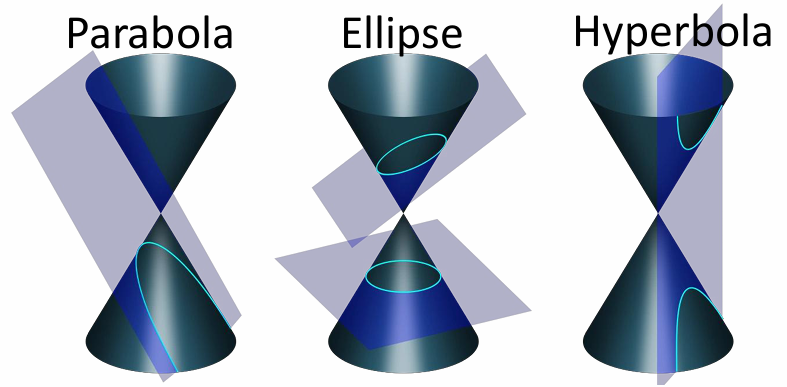
\includegraphics[width=0.7\linewidth]{images/conic sections.png}
    \end{center}
    \item For hyperbolas, we only need some qualitative properties in this course:
    \begin{itemize}
        \item Approaches 2 "linear asymptopes"
        \item Described by equation $x^2/a^2 - y^2/b^2 = 1$
    \end{itemize}
    \begin{center}
        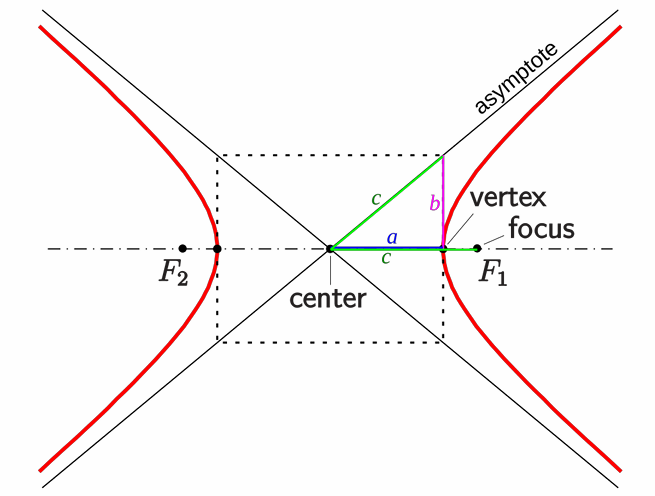
\includegraphics[width=0.5\linewidth]{images/hyperbola.png}
    \end{center}
    \item Kepler's First Law
    \begin{center}
        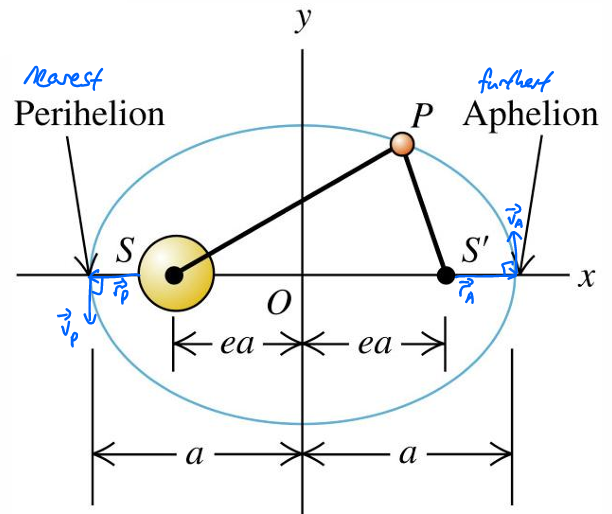
\includegraphics[width=0.6\linewidth]{images/kepler first law.png}
    \end{center}
    \begin{itemize}
        \item At perihelion and aphelion, $\vb{r} \perp \vb{v}$
        \item When $e = 0$, we have a circle
        \item When $e \rightarrow 1$, it approaches a "flat" ellipse
    \end{itemize}
    \item Kepler's First Law, Extended
    \begin{itemize}
        \item Solve DE for attractive inverse-square central force $\vb{\ddot{r}} = -\frac{GM}{r^2}\vb{r}$
        \item All solutions of this DE are conic sections (except trivial case where angular momentum $L = 0$)
        \item $K + U < 0$ ellipses (bound orbits)
        \item $K + U > 0$ hyperbola (unbound "orbits", approaches constant-velocity motion)
        \item $K + U = 0$ parabola (just "barely" unbounded: $v_{\text{esc}}$ is one example)
    \end{itemize}
    \item Kepler's Second Law (refer to Central Forces chapter)
    \item Kepler's Third Law: The square of the orbital period is proportional to the cube of the semi-major axis of the elliptical orbit, $T^2 = \frac{4\pi^2a^3}{GM}$
    \item General proof:
    \begin{center}
        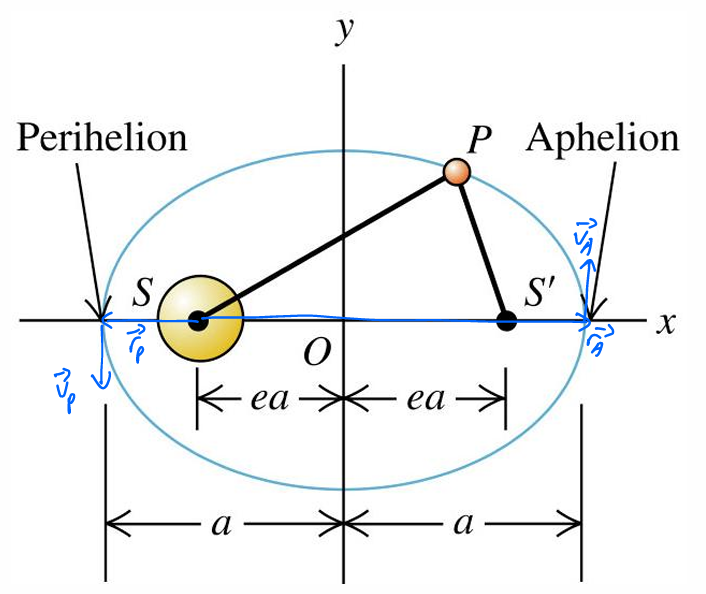
\includegraphics[width=0.6\linewidth]{images/kepler third law.png}
    \end{center}

    Use Second Law result: $\dv{A}{t} = \frac{L}{2m} \Rightarrow A = \frac{LT}{2m}$, so our goal is to find $\frac{L}{m}$ \\
    CoAM: $\frac{L}{m} = v_Pr_P = v_Ar_A \Rightarrow v_P = \frac{L}{mr_P}$ \\
    CoE:
    \[
    \begin{aligned}
        &\frac{E}{m} = \frac{1}{2}v_P^2 - \frac{GM}{r_P} = \frac{1}{2}v_A^2 - \frac{GM}{r_A} \\
        \Rightarrow &\frac{1}{2}\left(\frac{L}{mr_P}\right)^2 - \frac{GM}{r_P} = \frac{1}{2}\left(\frac{L}{mr_A}\right)^2 - \frac{GM}{r_A} \\
        \Rightarrow &\left(\frac{L}{m}\right)^2 \left(\frac{1}{r_P^2} - \frac{1}{r_A^2}\right) = 2GM \left(\frac{1}{r_P} - \frac{1}{r_A}\right) \\
        \Rightarrow &\left(\frac{L}{m}\right)^2 = 2GM\left( \frac{1}{r_P} + \frac{1}{r_A} \right)^{-1} = 2GM\left(\frac{r_Pr_A}{r_P + r_A}\right)
    \end{aligned}
    \]
    For eccentricity definition, $r_P = (1 - e)a$ and $r_A = (1 + e)a$, so \\
    \[
    \begin{aligned}
        \left(\frac{L}{m}\right)^2 &= 2GM\left(\frac{r_Pr_A}{r_P + r_A}\right) \\
        &= 2GM\left(\frac{(1-e^2)a^2}{2a}\right) \\
        &= GMa(1 - e^2)
    \end{aligned}
    \]
    Sub $A = \frac{LT}{2m}$, rearrange to get $T^2 = \frac{4A^2}{GMa(1-e^2)}$ \\
    Recall: $A = \pi ab$, \\
    New fun fact: $b^2 = a^2 - c^2 = a^2(1 - e^2)$ \\
    Hence, $T^2 = \frac{4(\pi ab)^2}{GMb^2/a} = \frac{4\pi^2a^3}{GM}$    
\end{itemize}

\end{multicols*}
\end{document}